\documentclass{article}

\usepackage[margin=1in]{geometry}
\usepackage[section]{placeins}
\usepackage[colorlinks,bookmarks,bookmarksnumbered,citecolor=red,urlcolor=red]{hyperref}
\usepackage{graphicx}
\usepackage[caption=false]{subfig}
\usepackage{amsmath}
\usepackage{cleveref}  % must load after hyperref
% \usepackage[noabbrev]{cleveref}  % must load after hyperref

\begin{document}

\author{S. Andrew Ning}
\title{Vertical Axis Wind Turbine Aerodynamics Analysis}
% \title{Double Multiple Streamtube Method}
\maketitle

\section{Introduction}

This paper discussed two approaches for analyzing the aeordynamics of vertical axis wind turbines (VAWTs): the double multiple streamtube model \cite{Paraschivoiu1983}, and the actuator cylinder flow model \cite{Madsen1982, Madsen2013}.  The presentation of the methodologies are modified slightly in this document to account for blade curvature and sweep, and to utilize a common coordinate system and variable naming.  The coordinate system used in shown in \Cref{fig:coordinate}.

\begin{figure}[htbp]
\begin{center}
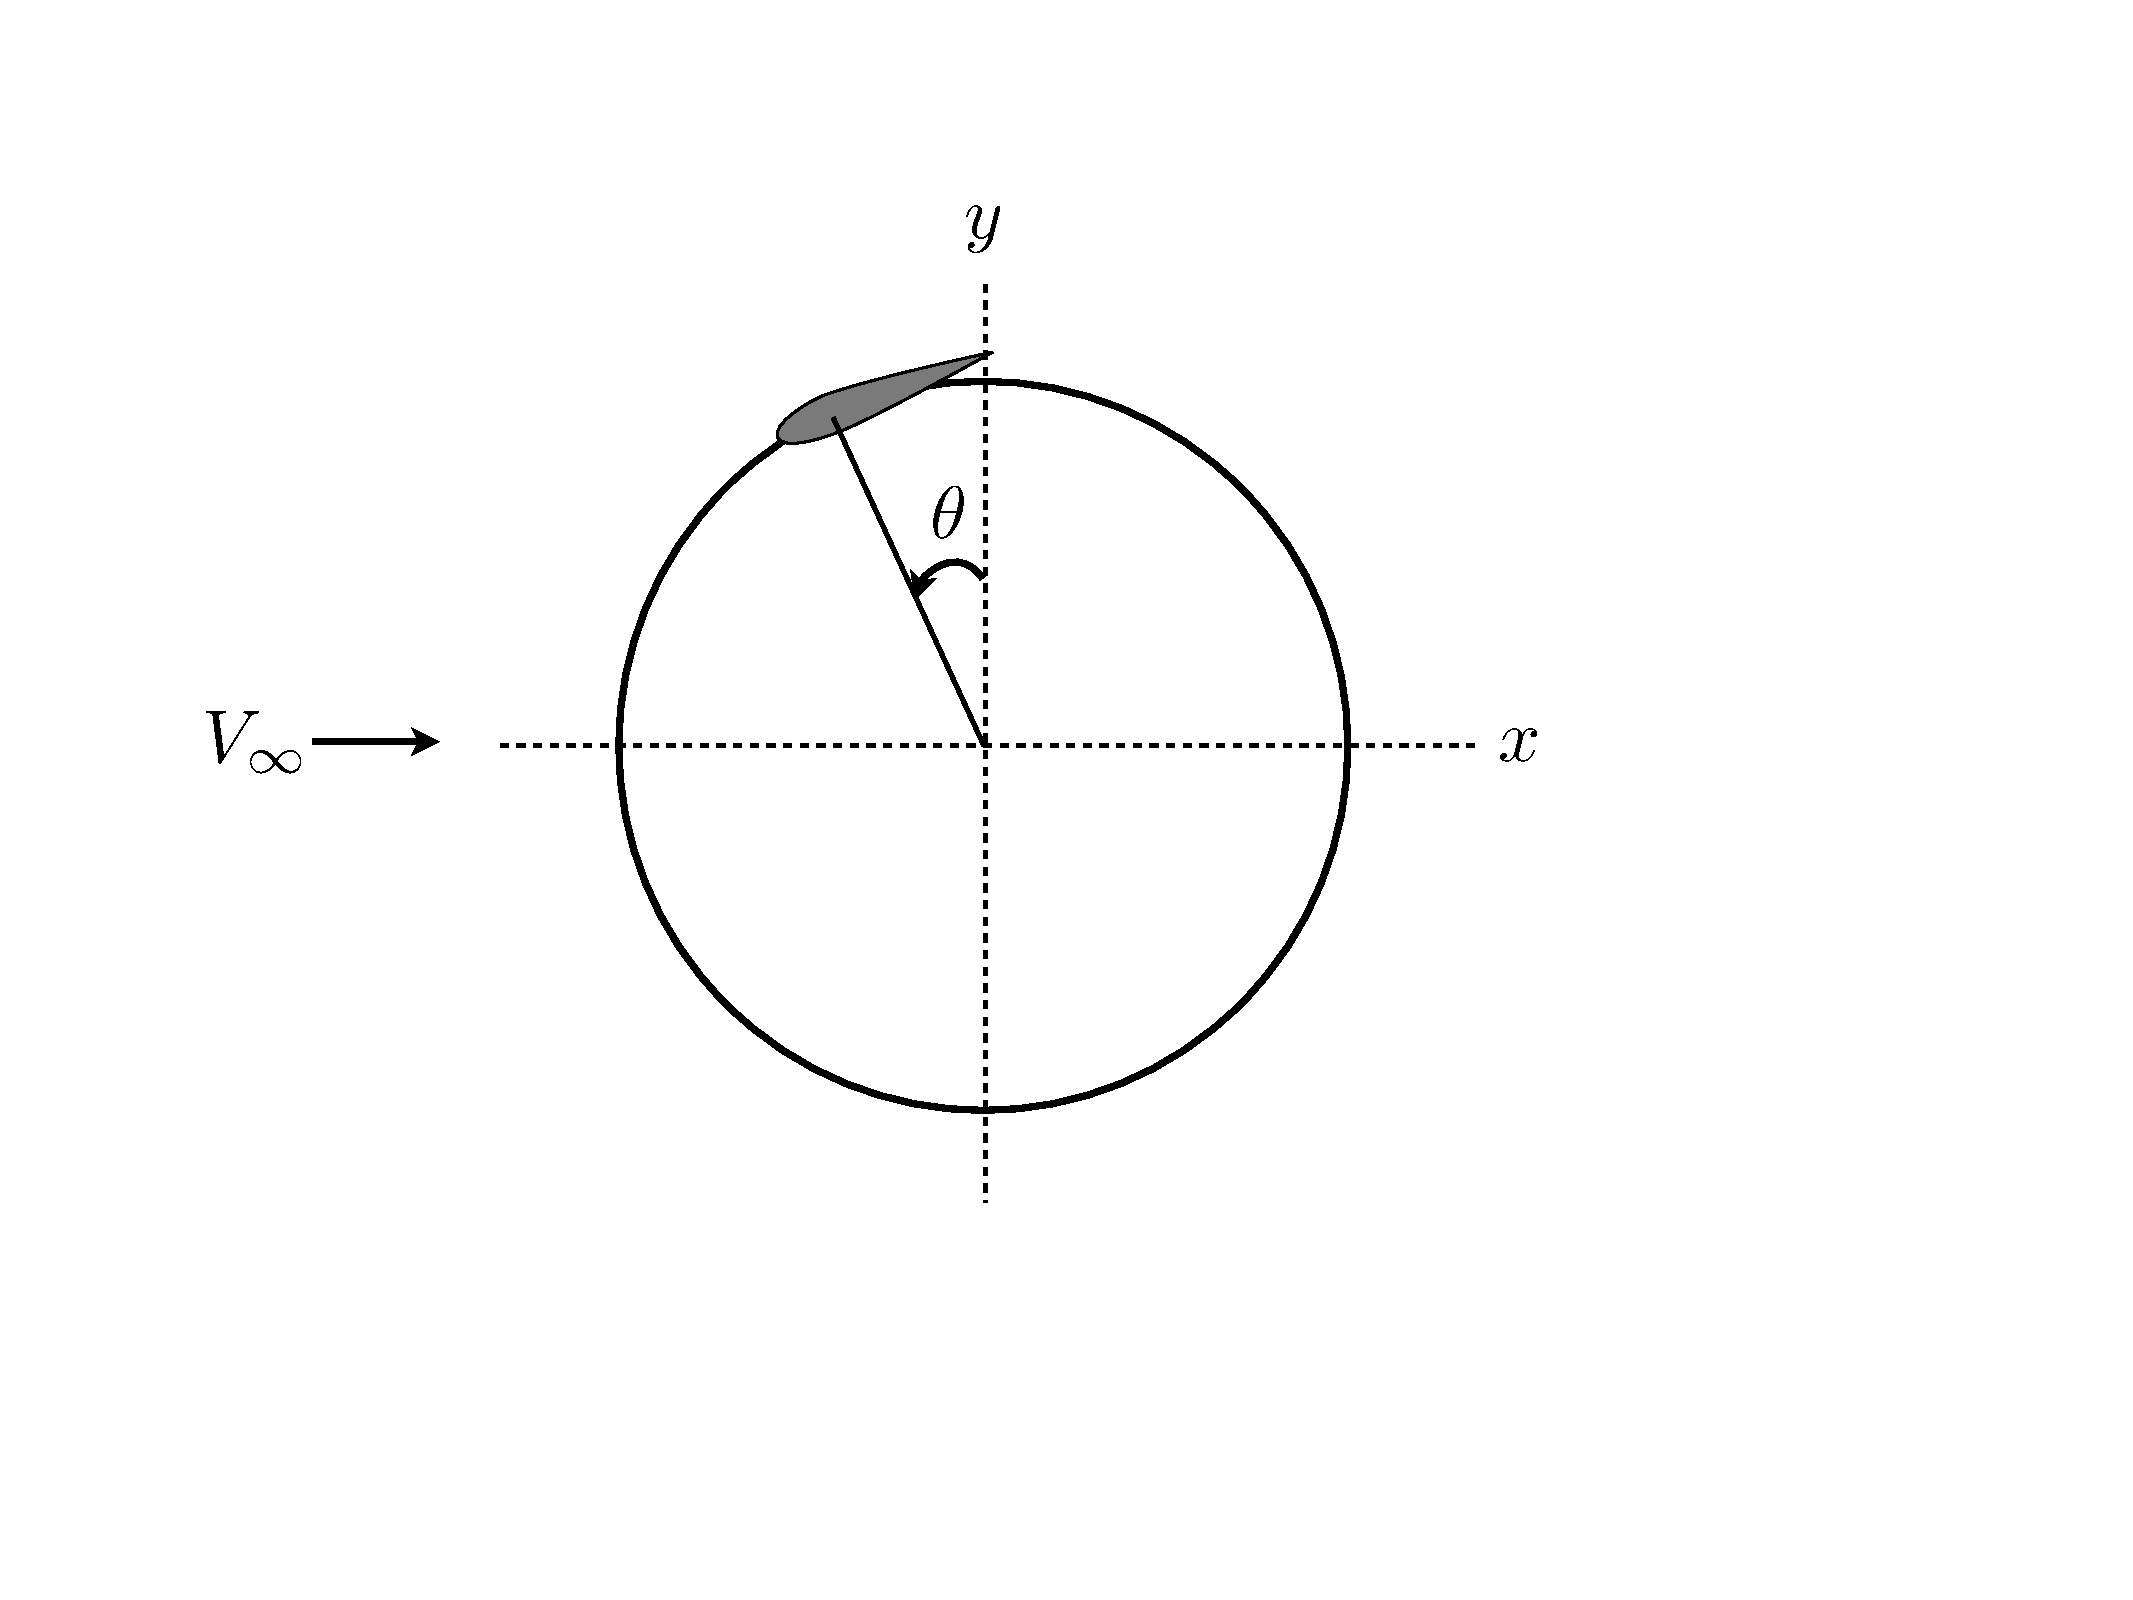
\includegraphics[width=3.5in]{images/coordinate}
\caption{Coordinate system used in following methodologies.}
\label{fig:coordinate}
\end{center}
\end{figure}

\section{Double Multiple Streamtube Model}
\label{sec:dmst}

Conceptual aerodynamic analysis of horizontal axis wind turbines (HAWTs) begins with actuator disk theory.  In this theory the swept area of the rotor is idealized as an infinitely thin disk across which a one-dimensional streamtube of air experiences a pressure drop (Figure \ref{fig:actuatordisk}).  Based on these simple assumptions, thrust and power can be estimated using conservation of mass, momentum, and energy.

\begin{figure}[htbp]
\begin{center}
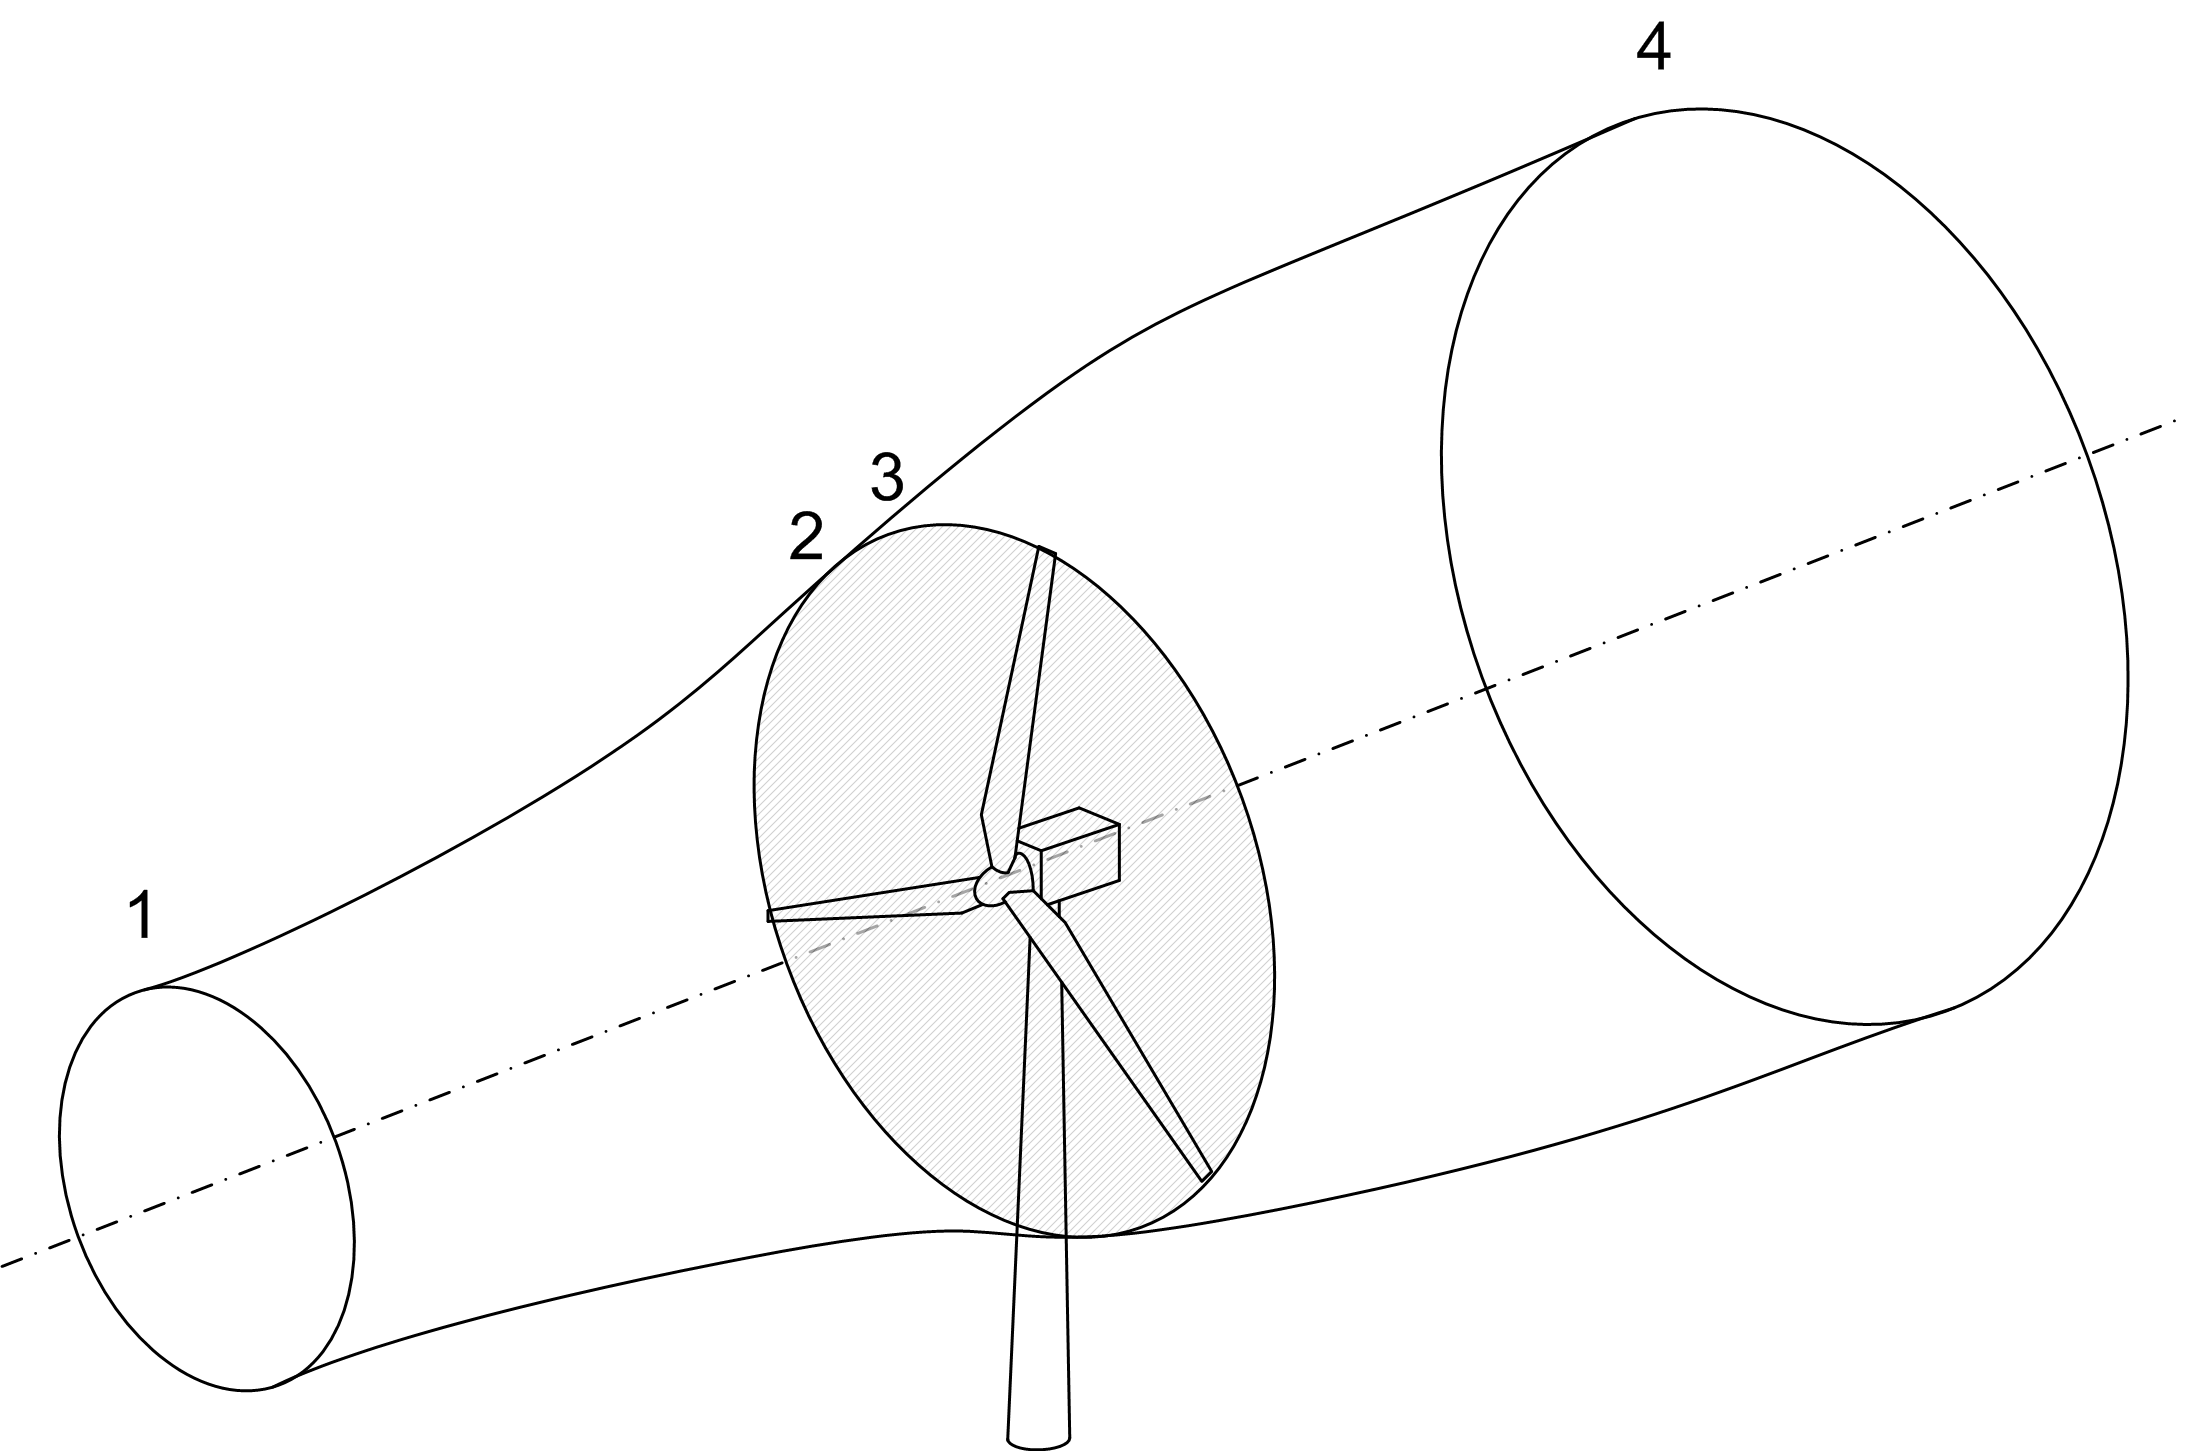
\includegraphics[width=3.5in]{images/actuatordisk}
\caption{The actuator disk (from 2 to 3) concept used in modeling aeordynamic performance of horizontal axis wind turbines.  [need to find ref]}
\label{fig:actuatordisk}
\end{center}
\end{figure}

Streamtube theory attempts to apply the same concept to VAWT aerodynamic performance estimation.  Each cross-section of the VAWT (constant height) is approximated as an actuator disk in the mid-plane (essentially a cross-plane actuator line for the 2D slice). However, constant flow parameters across the entire disk is too coarse of a model for this application because the relative velocity changes significantly as the blades rotate around the vertical axis.  The natural extension of this theory is multiple streamtube theory where instead of using one large streamtube passing through the actuator disk, the actuator disk is discretized into multiple streamtubes across with independent induction factors (see \Cref{fig:top} for an example of one streamtube in a multiple streamtube model).  An additional extension, double multiple streamtube theory, utilizes two actuator disks to represent the upstream and downstream sides of the cylinder.  While this is still a coarse approximation of the actual swept surface of a VAWT it is clearly an improvement over single streamtube and/or single actuator disk models.

\subsection{Methodology}
At a given height $z$ the two actuator disks are allowed to have separate momentum losses at both the upstream and downstream surfaces.  It is assumed that after passing through the first surface, the velocity reaches its far-field value before reaching the second surface.  Thus, using actuator disk theory and referring to \Cref{fig:top} the velocities are given as
\begin{align}
V &= V_\infty (1-a) \label{eq:V}\\
V_e &= V_\infty (1-2a) \label{eq:Ve}\\
V^\prime &= V_e (1-a^\prime) \label{eq:Vprime}
\end{align}

\begin{figure}[htbp]
\begin{center}
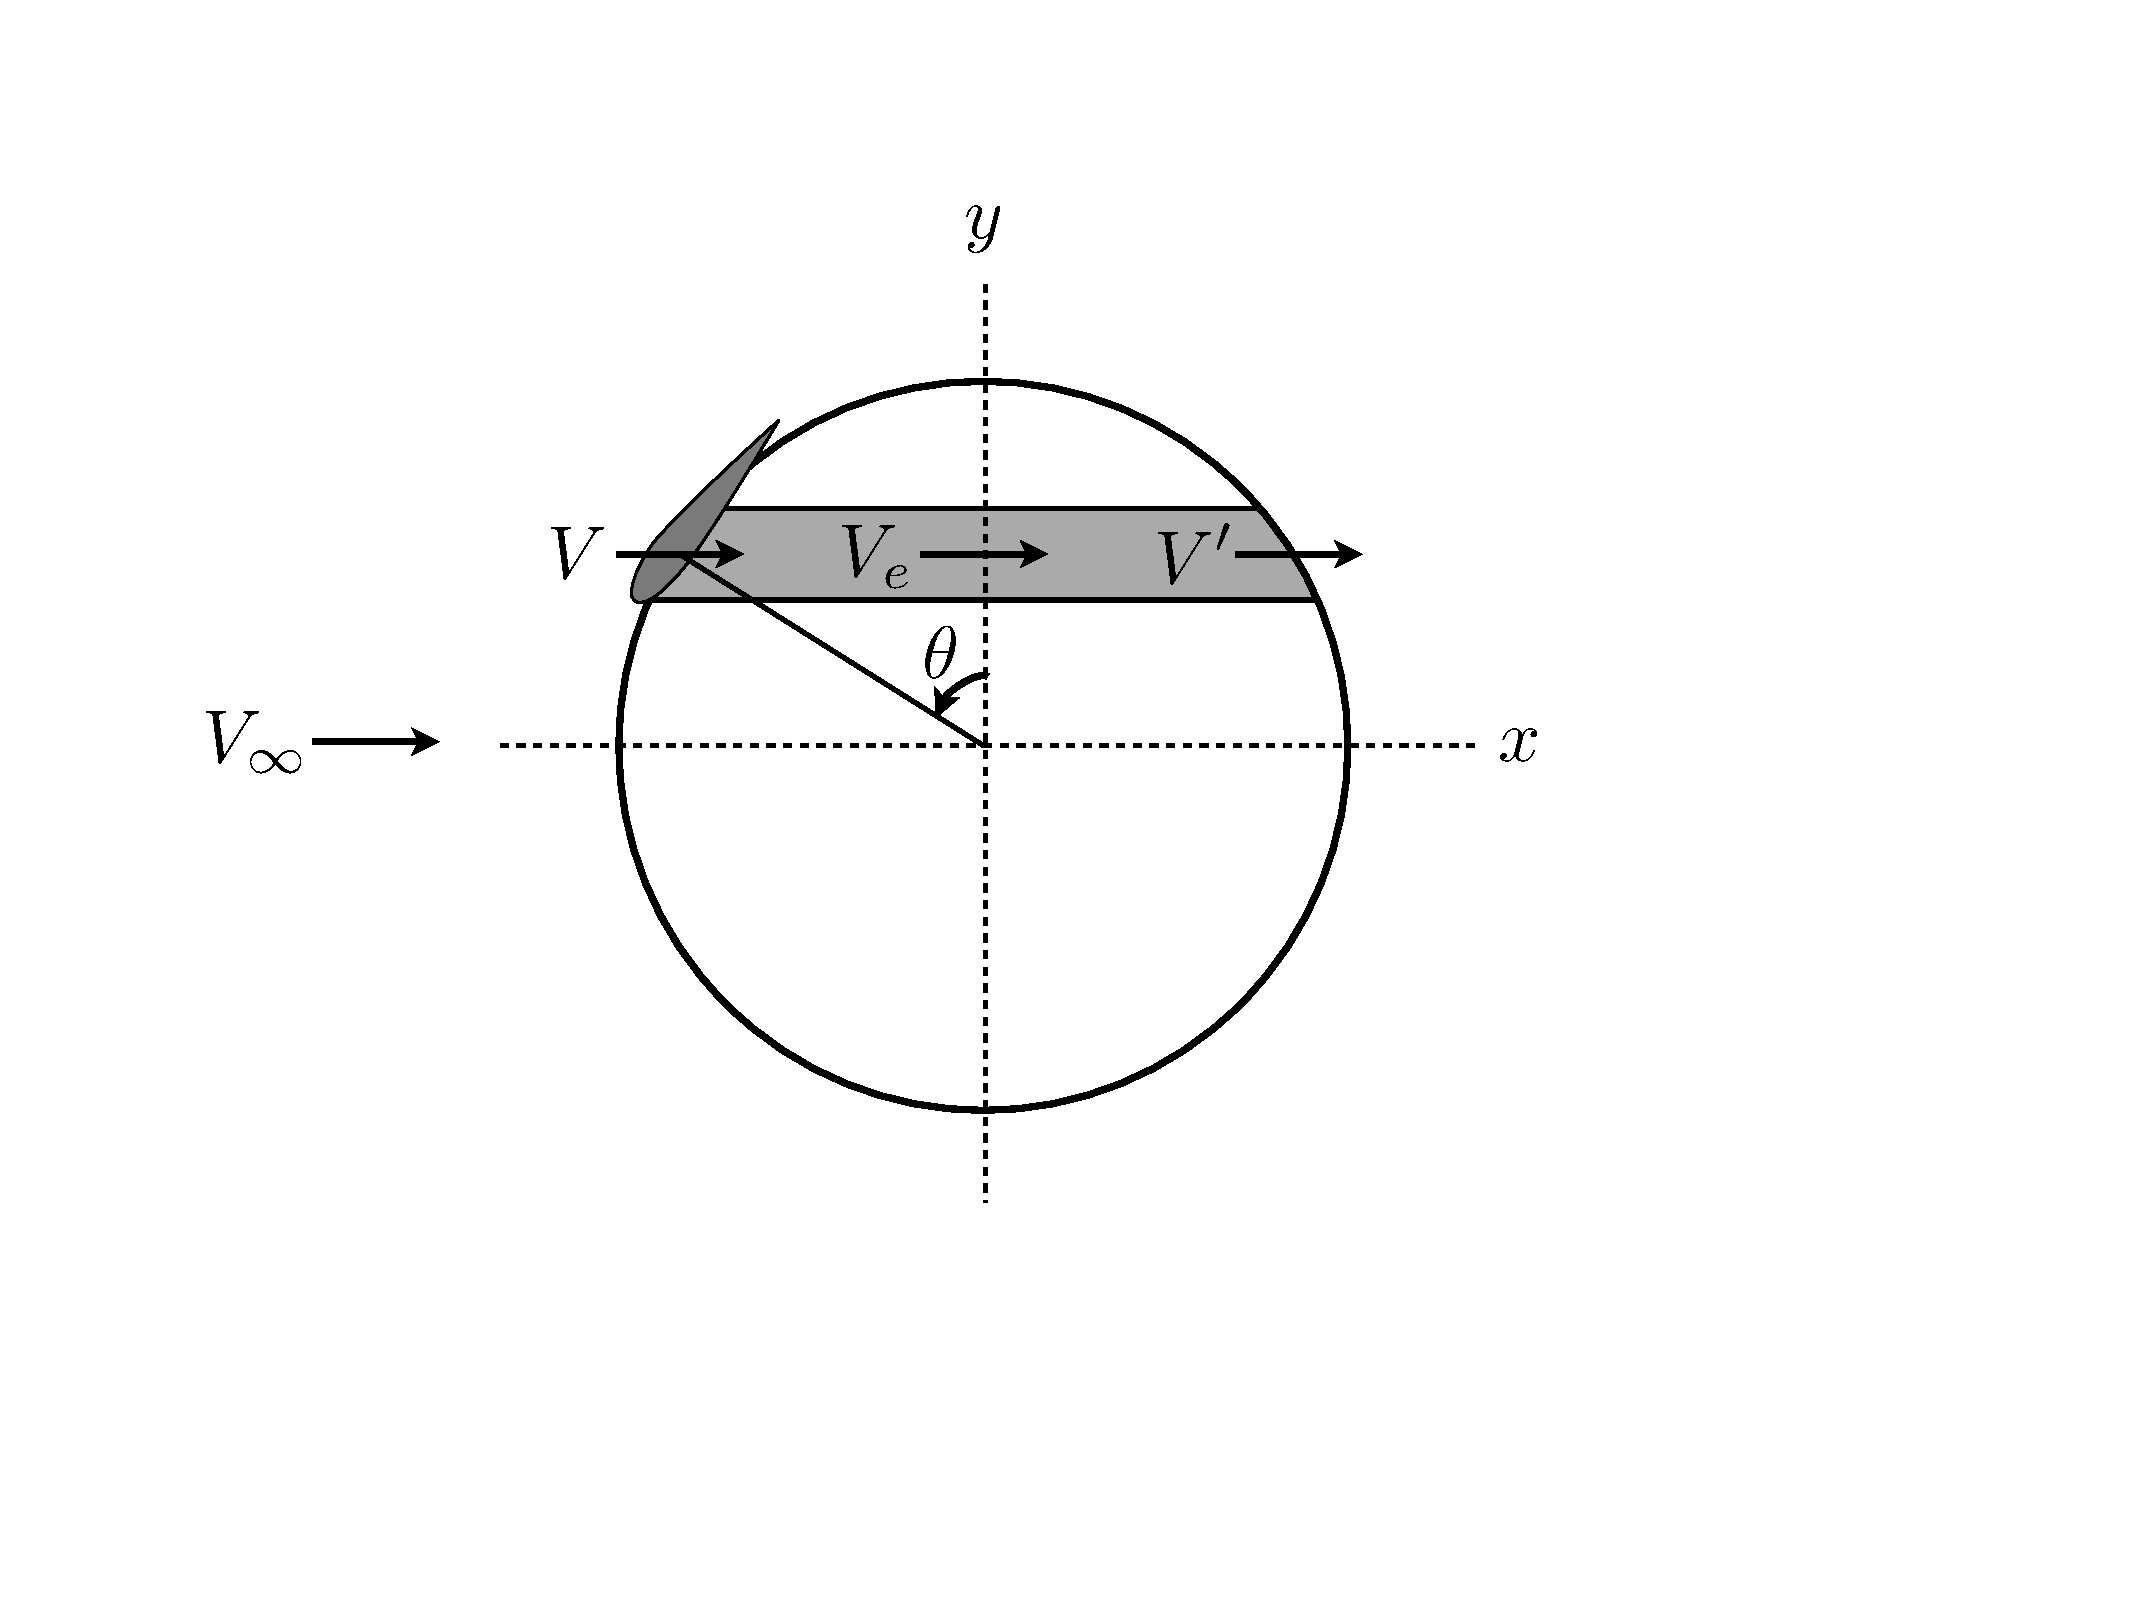
\includegraphics[width=4in]{images/top}
\caption{Top view of VAWT showing momentum losses at upstream and downstream portion of streamtube (only one blade shown).}
\label{fig:top}
\end{center}
\end{figure}

\subsection{Momentum Theory}
Referring to \Cref{fig:top} we see that the mass flow rate in the streamtube is
\begin{equation}
\dot{m} = \rho V \Delta A
\end{equation}
where $\Delta A$ is the cross-sectional area of the inlet to the streamtube.  Referring to \Cref{fig:da} we see that for some distance $\Delta z$ in the z-direction the cross-sectional inlet area is
\begin{equation}
\Delta A = r \Delta \theta |\sin\theta| \Delta z
\label{eq:deltaA}
\end{equation}

\begin{figure}[htbp]
\begin{center}
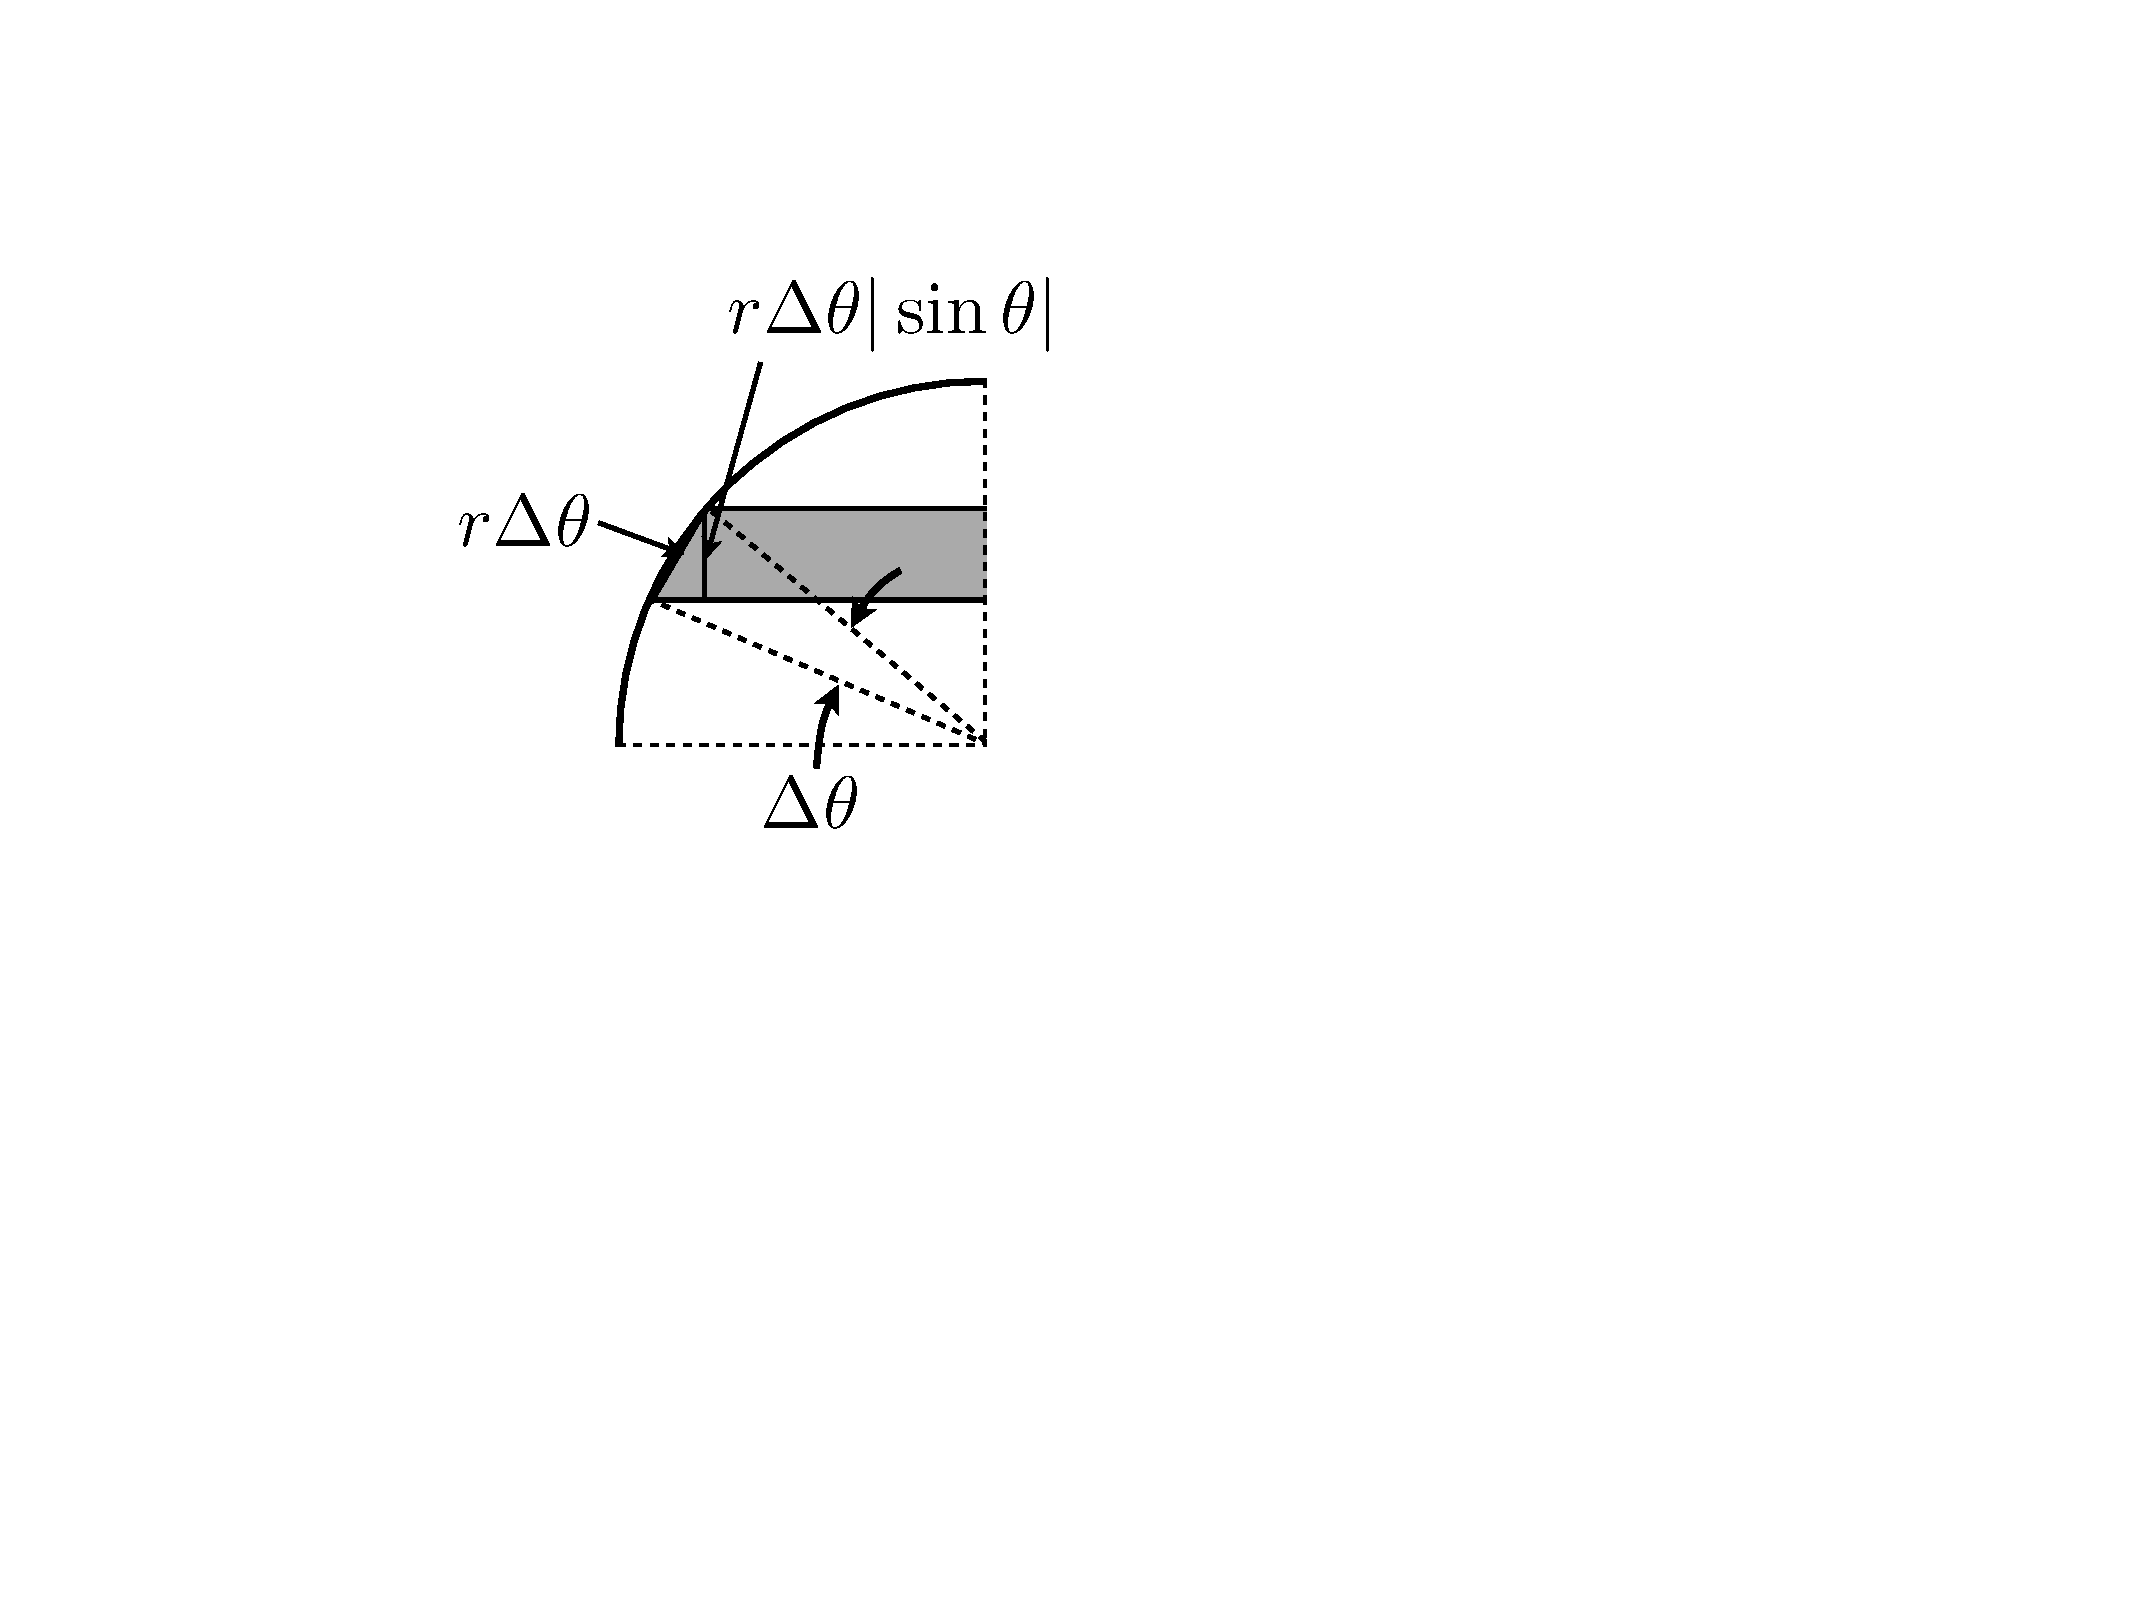
\includegraphics[width=2in]{images/da}
\caption{Width of streamtube at inlet.}
\label{fig:da}
\end{center}
\end{figure}


Applying the momentum equation across the first actuator disk yields
\begin{equation}
    T = \rho V \Delta A (V_\infty - V_e)
\end{equation}
Using Equations \eqref{eq:V} and \eqref{eq:Ve}, and normalizing by the freestream dynamic pressure and $\Delta A$ yields the familiar equation
\begin{equation}
    C_T = 4a(1-a)
    \label{eq:ctmom}
\end{equation}
For induction factors larger than $0.4$ we can utilize Buhl's modification to Glauert's correction
\begin{equation}
    C_T = \frac{2}{9} (7a^2 - 2a + 4)
    \label{eq:ctglauert}
\end{equation}


\subsection{Blade Element Theory}

Looking at just the upstream surface for the moment, from \Cref{fig:Vtop} we see that the external velocity is composed of a horizontal component and a rotation component
\begin{equation}
    V_{ext} = V\hat{x} - \Omega r \hat{t}
\end{equation}
Transforming the horizontal component into the $(\hat{r}, \hat{t})$ coordinate system we get
\begin{equation}
    V_{ext} = -(V\sin\theta)\hat{r} - (\Omega r + V\cos\theta) \hat{t}
\end{equation}

\begin{figure}[htbp]
\centering
 \subfloat[Top view of incoming velocity and rotational velocity.]{
   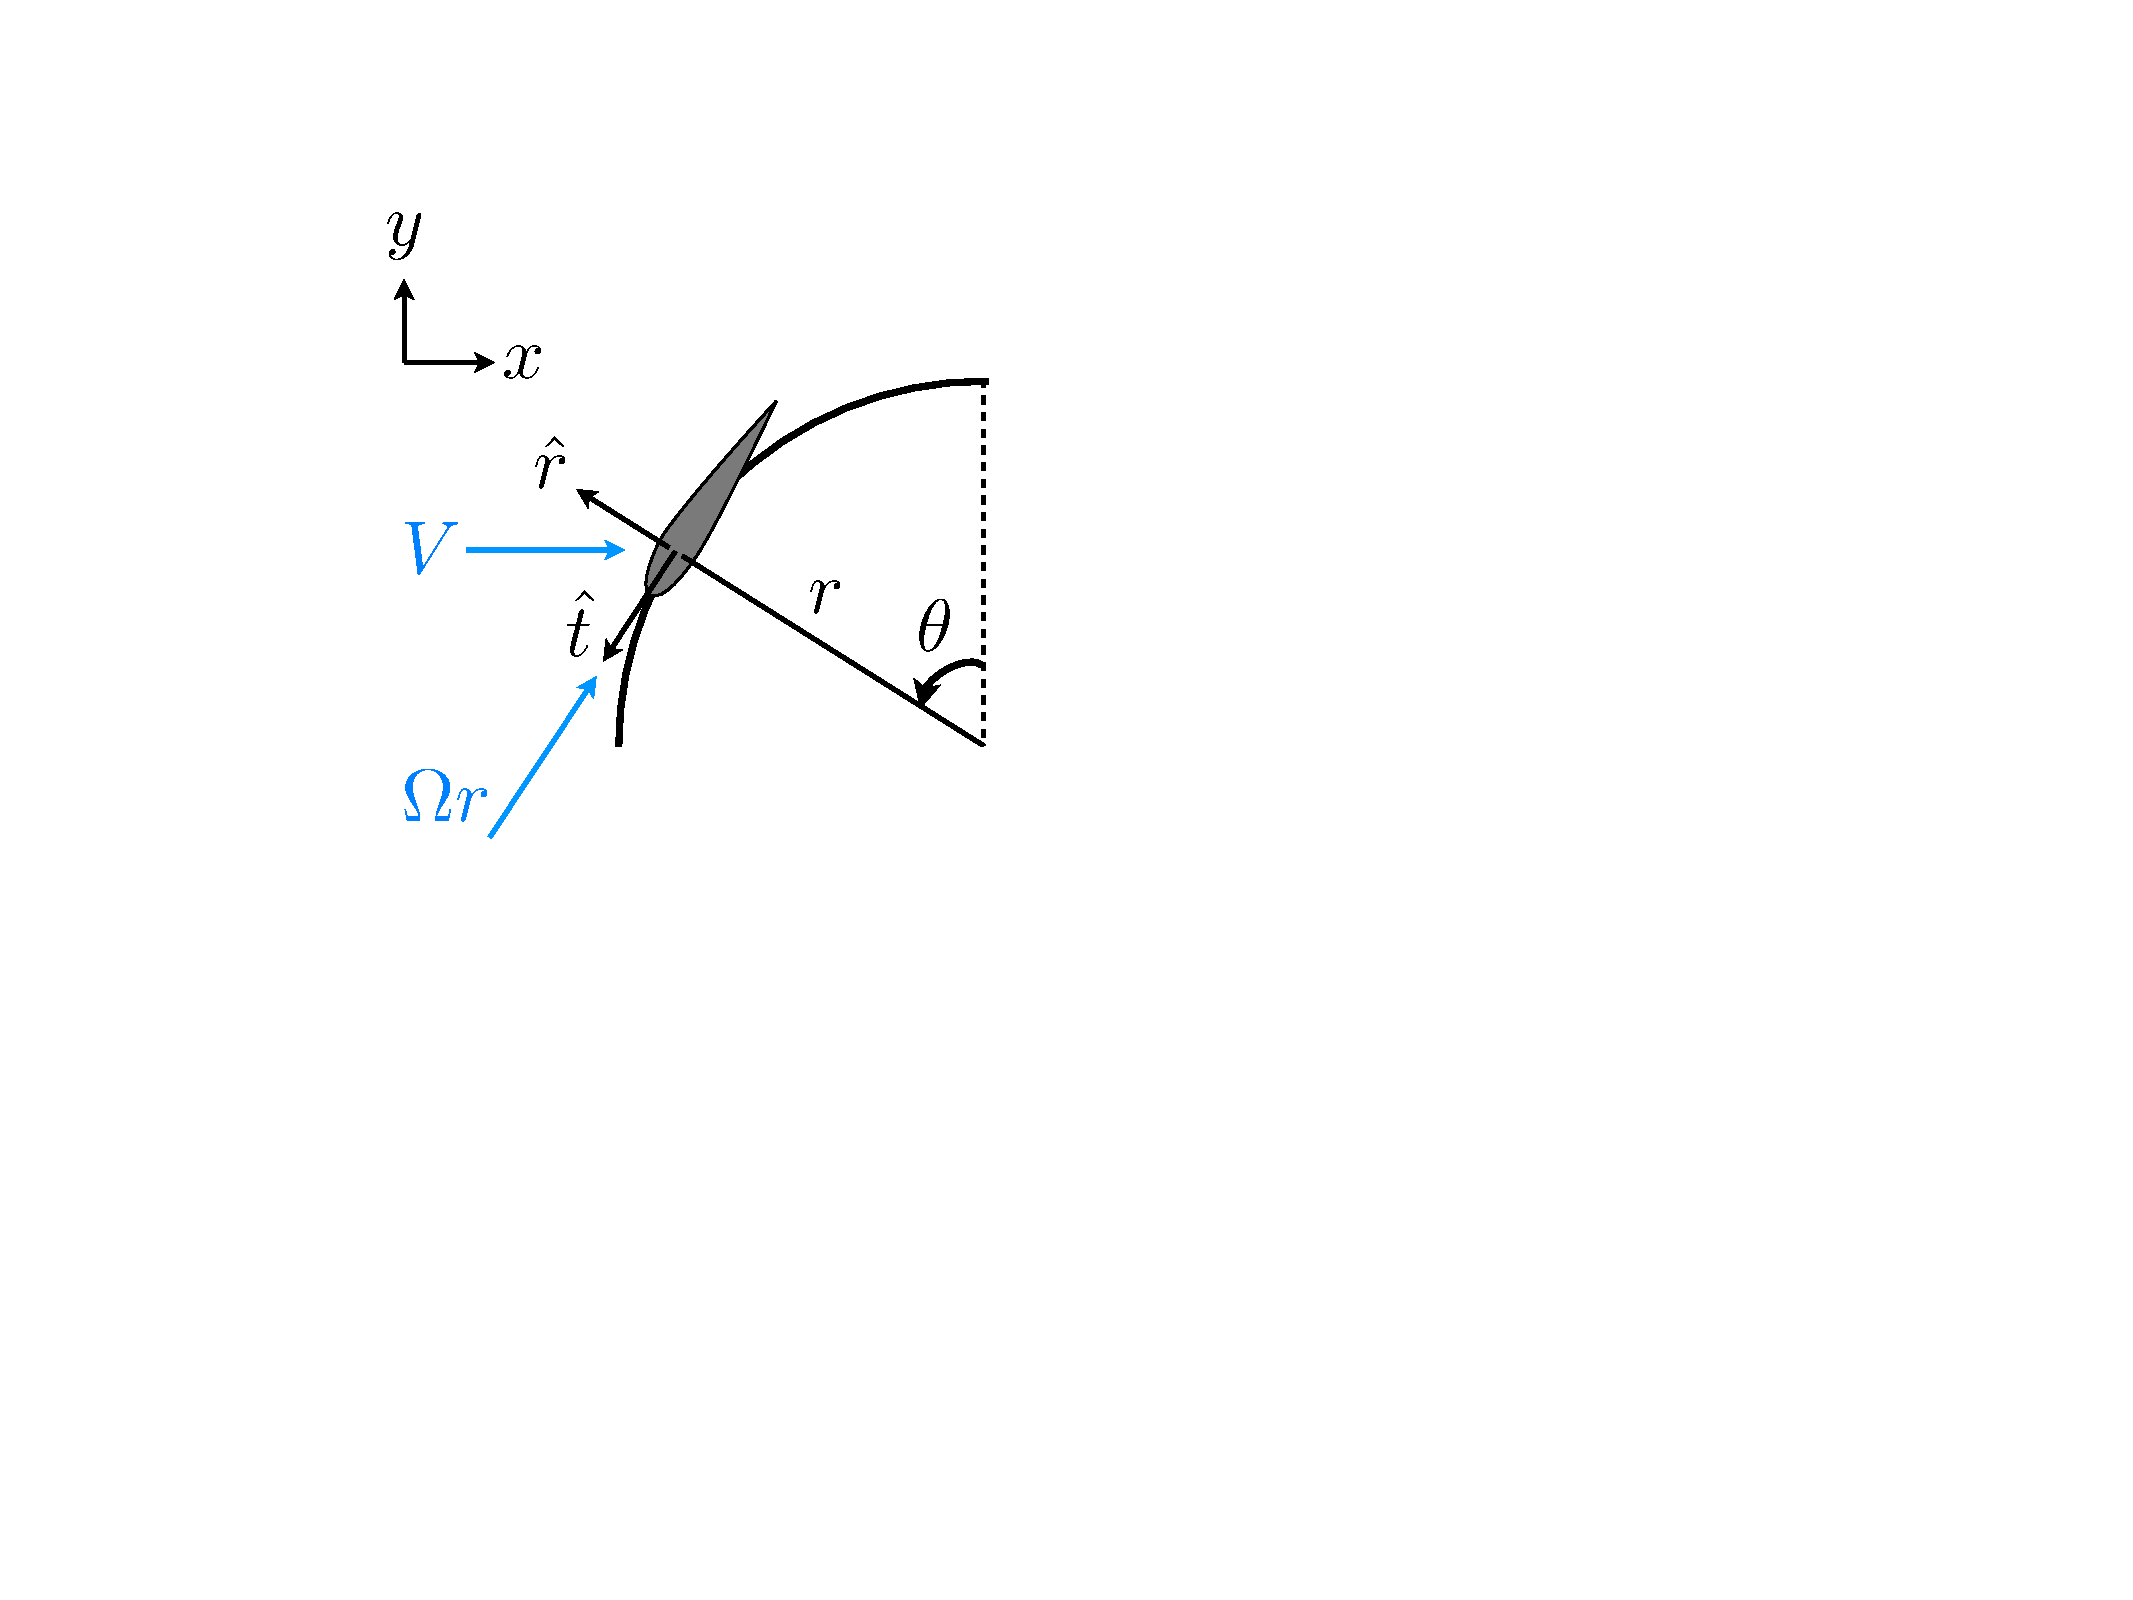
\includegraphics[width=0.4\textwidth]{images/Vtop}
   \label{fig:Vtop}
 }
 \qquad
 \subfloat[Side view with radial component of velocity shown.  Tangential component is into the page.]{
   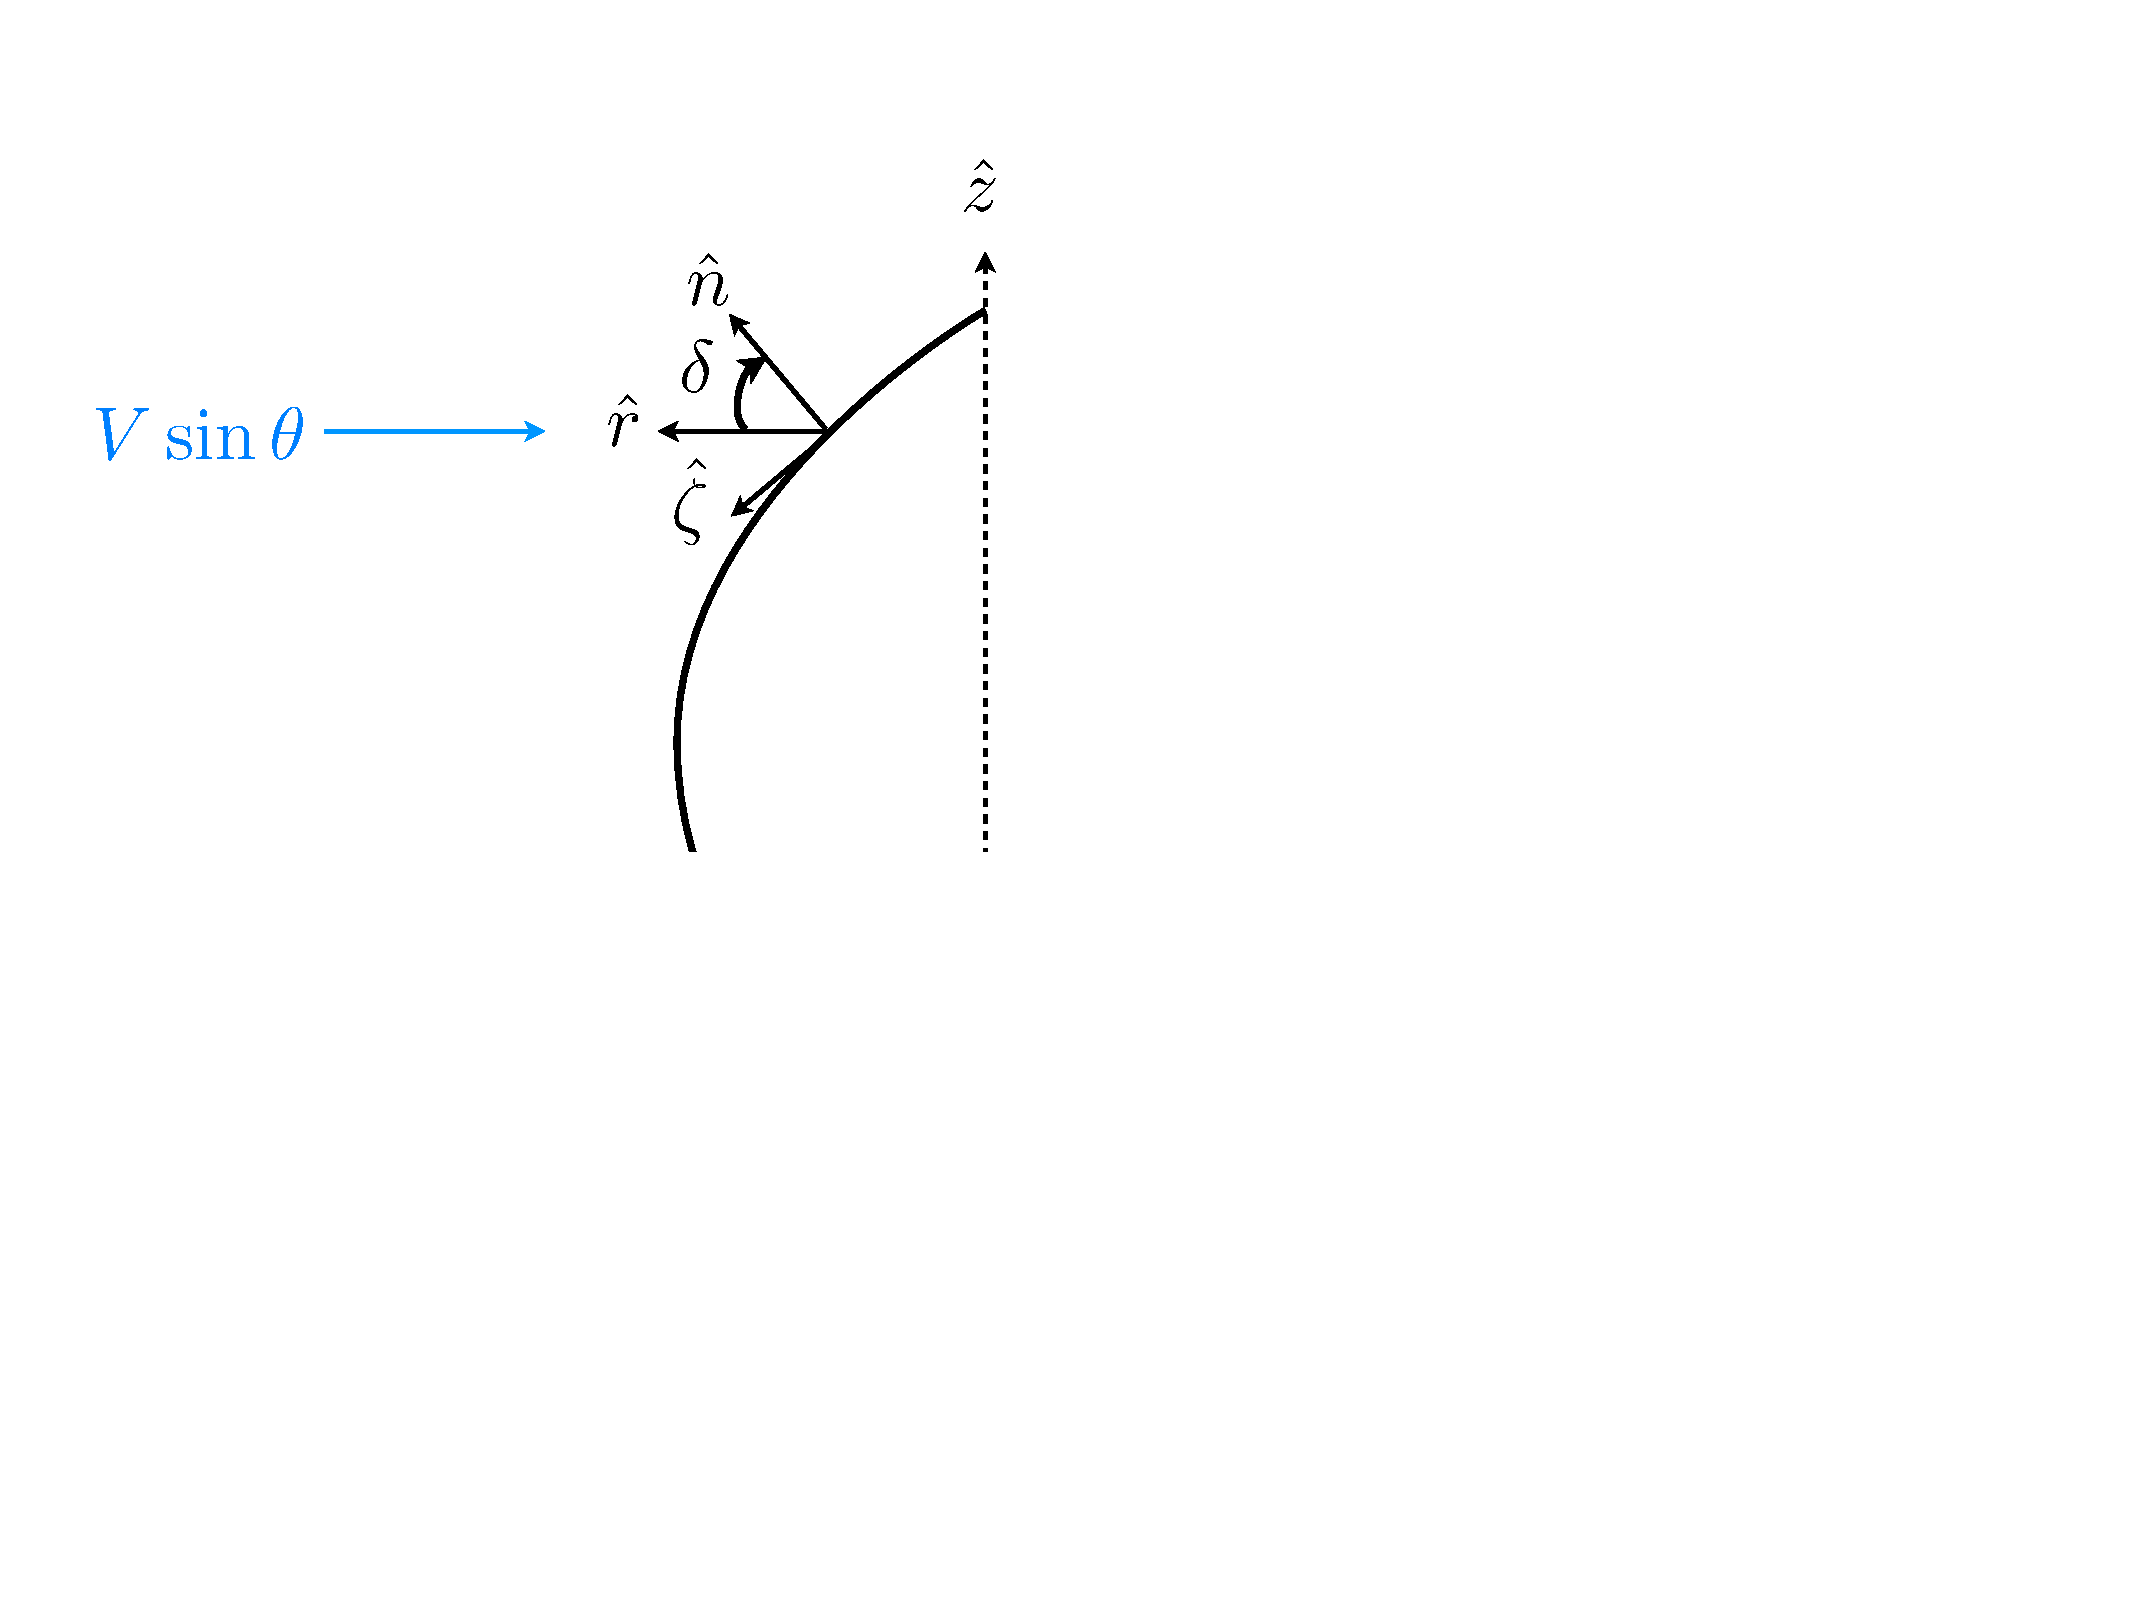
\includegraphics[width=0.5\textwidth]{images/Vside}
   \label{fig:Vside}
 }
 \caption{Top and side view of VAWT with incoming velocity components.}
\end{figure}


However, the blade may also be curved so from a side view (\Cref{fig:Vside}) we can further resolve the radial component of the velocity to a normal component and a cross-flow component.
\begin{equation}
    V_{ext} = -(V\sin\theta\cos\delta) \hat{n} - (V\sin\theta\sin\delta) \hat{\zeta} - (\Omega r + V\sin\theta) \hat{t}
\end{equation}
The blade may also be swept, however it is assumed that the sweep is accomplished through shearing rather than rotation. In other words, it assumed that the airfoils are still defined relative to the streamwise direction as opposed to normal to the local blade sweep.


The velocity components can now be resolved in the plane of the airfoil (spanwise flow is neglected in blade element momentum theory).  From \Cref{fig:Vairfoil} we see that the magnitude of the inflow velocity, the inflow angle, and the angle of attack are given as
\begin{equation}
\begin{aligned}
W &= \sqrt{(\Omega r + V \cos\theta)^2 + (V\sin\theta\cos\delta)^2}\\
\phi &= \tan^{-1}\left( \frac{V \sin\theta \cos\delta}{\Omega r + V \cos\theta}\right) \\
\alpha &= \phi - \beta
\label{eq:alpha}
\end{aligned}
\end{equation}


\begin{figure}[htbp]
\begin{center}
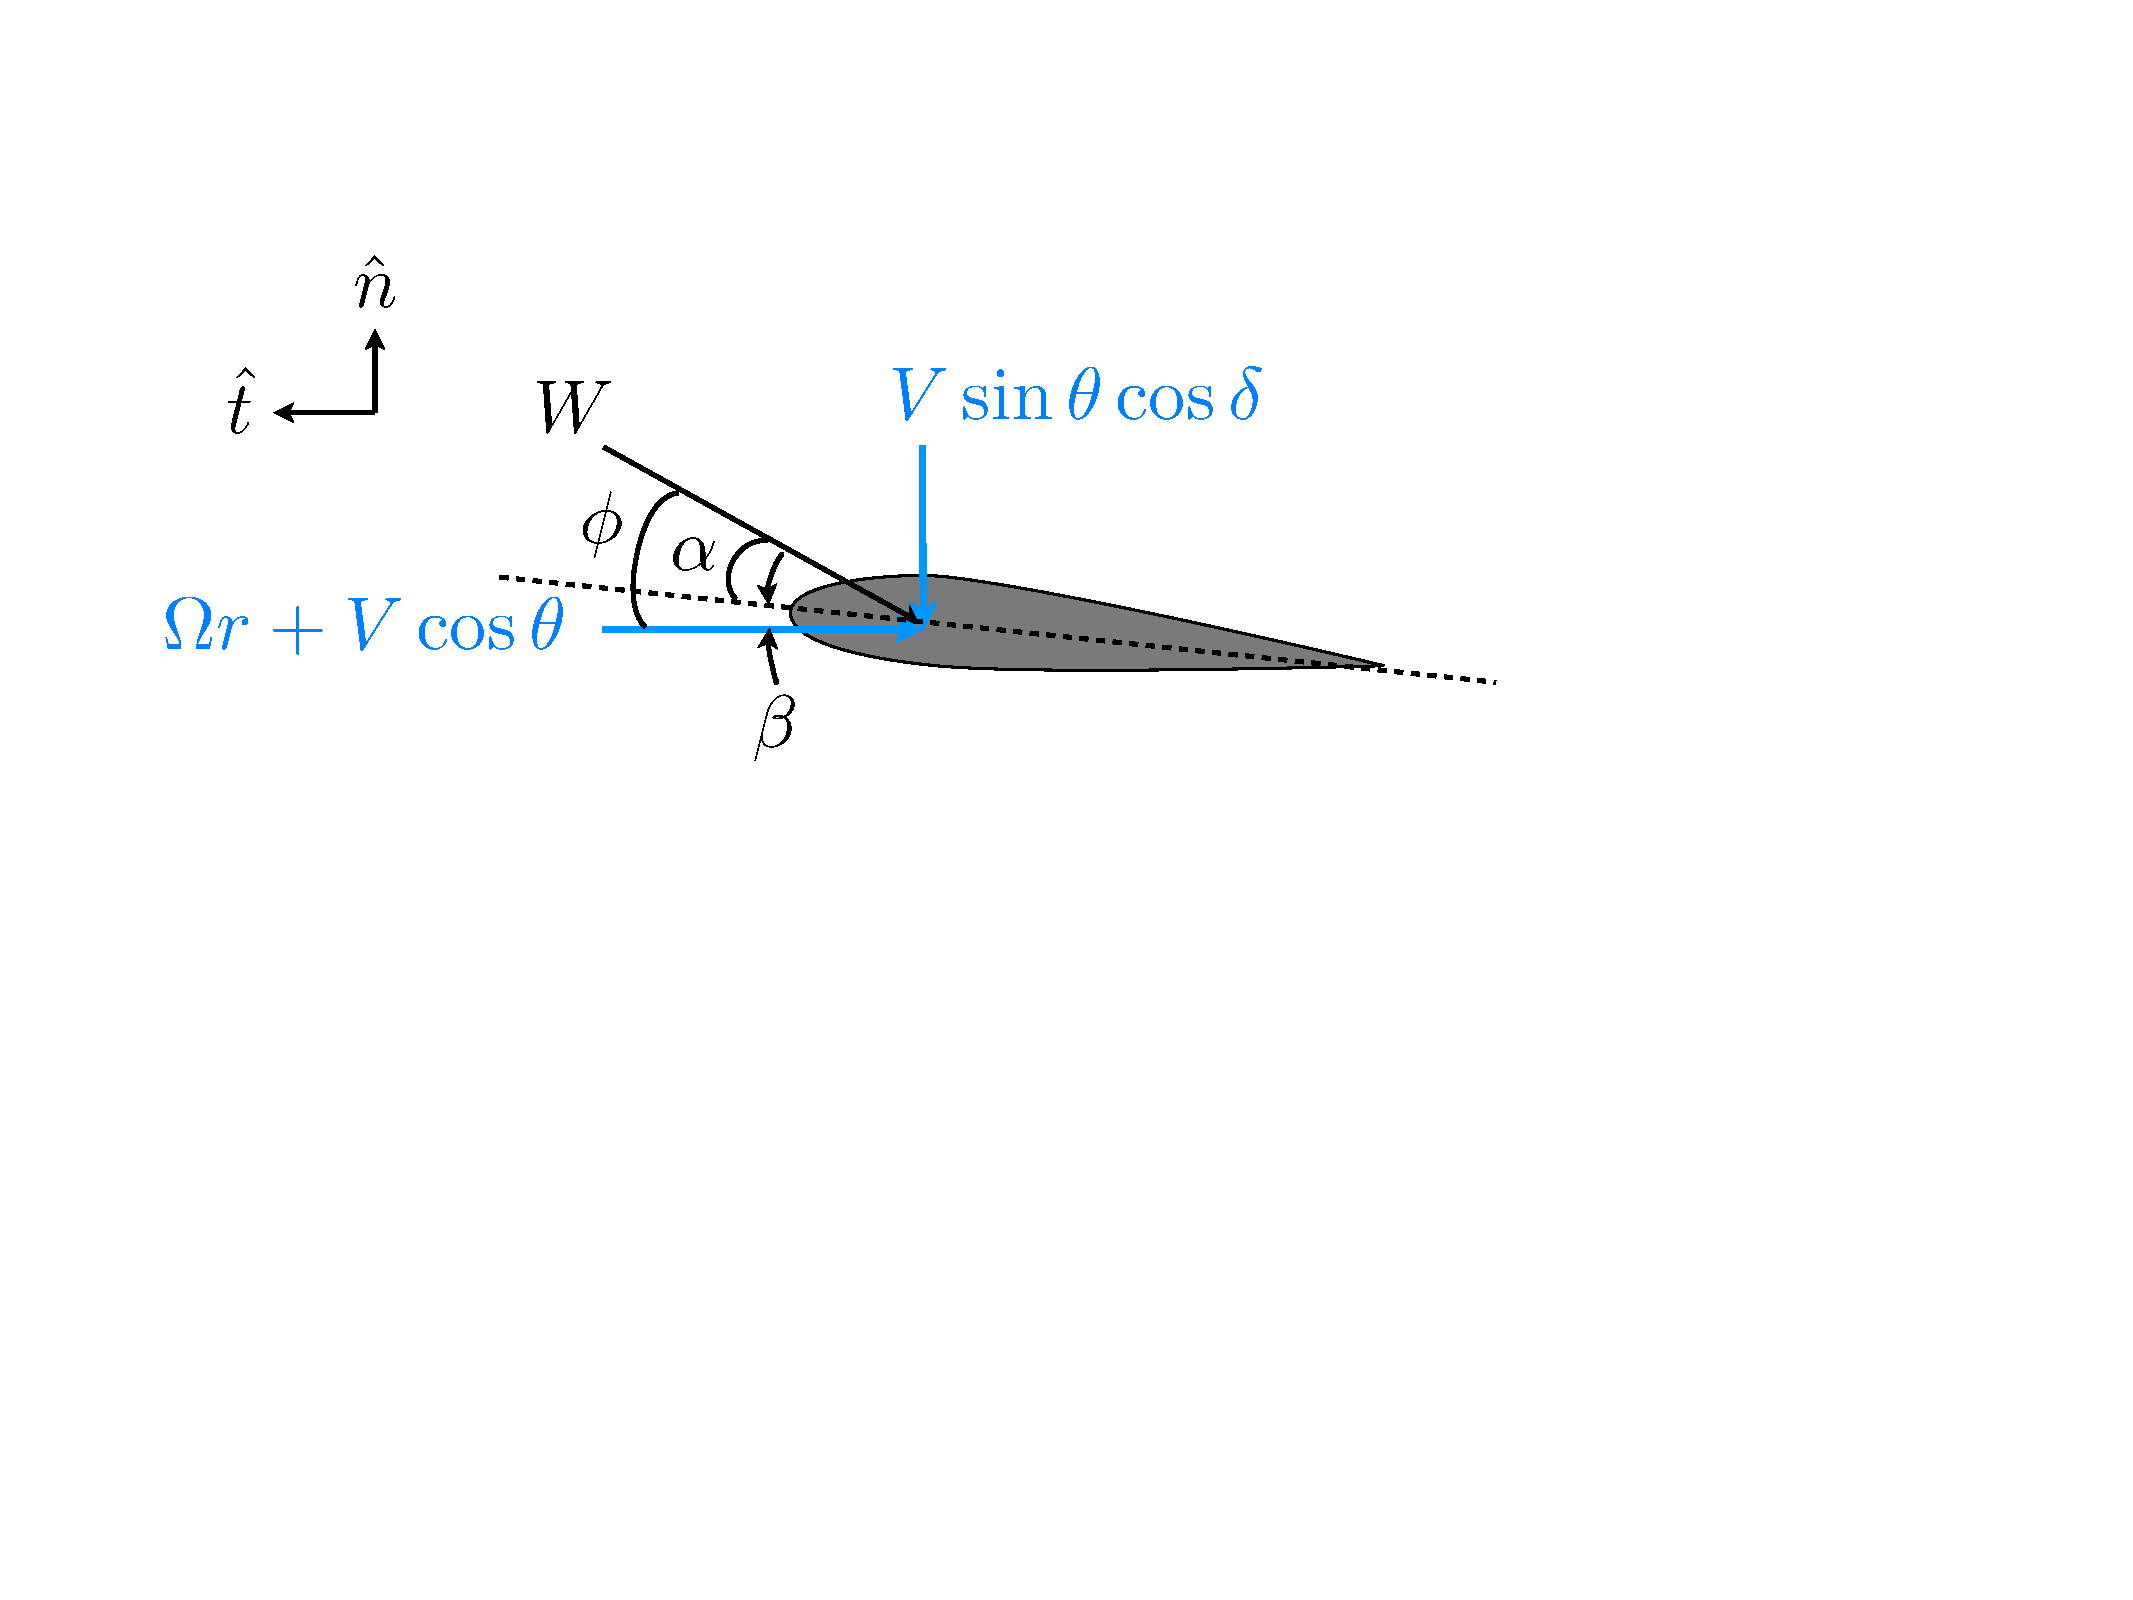
\includegraphics[width=3.5in]{images/Vairfoil}
\caption{Velocity components in the plane of the airfoil.  The cross-flow component of the velocity is into the page.}
\label{fig:Vairfoil}
\end{center}
\end{figure}


With the angle of attack and Reynolds number the airfoil lift and drag can be computed, and then rotated into the normal and tangential force coefficients (note that $c_n$ is defined as positive in the opposite direction of $\hat{n}$ in \Cref{fig:cn}).

\begin{equation}
\begin{aligned}
c_n &= c_l \cos\phi + c_d\sin\phi \\
c_t &= c_l \sin\phi - c_d\cos\phi
\label{eq:cn}
\end{aligned}
\end{equation}

\begin{figure}[htbp]
\begin{center}
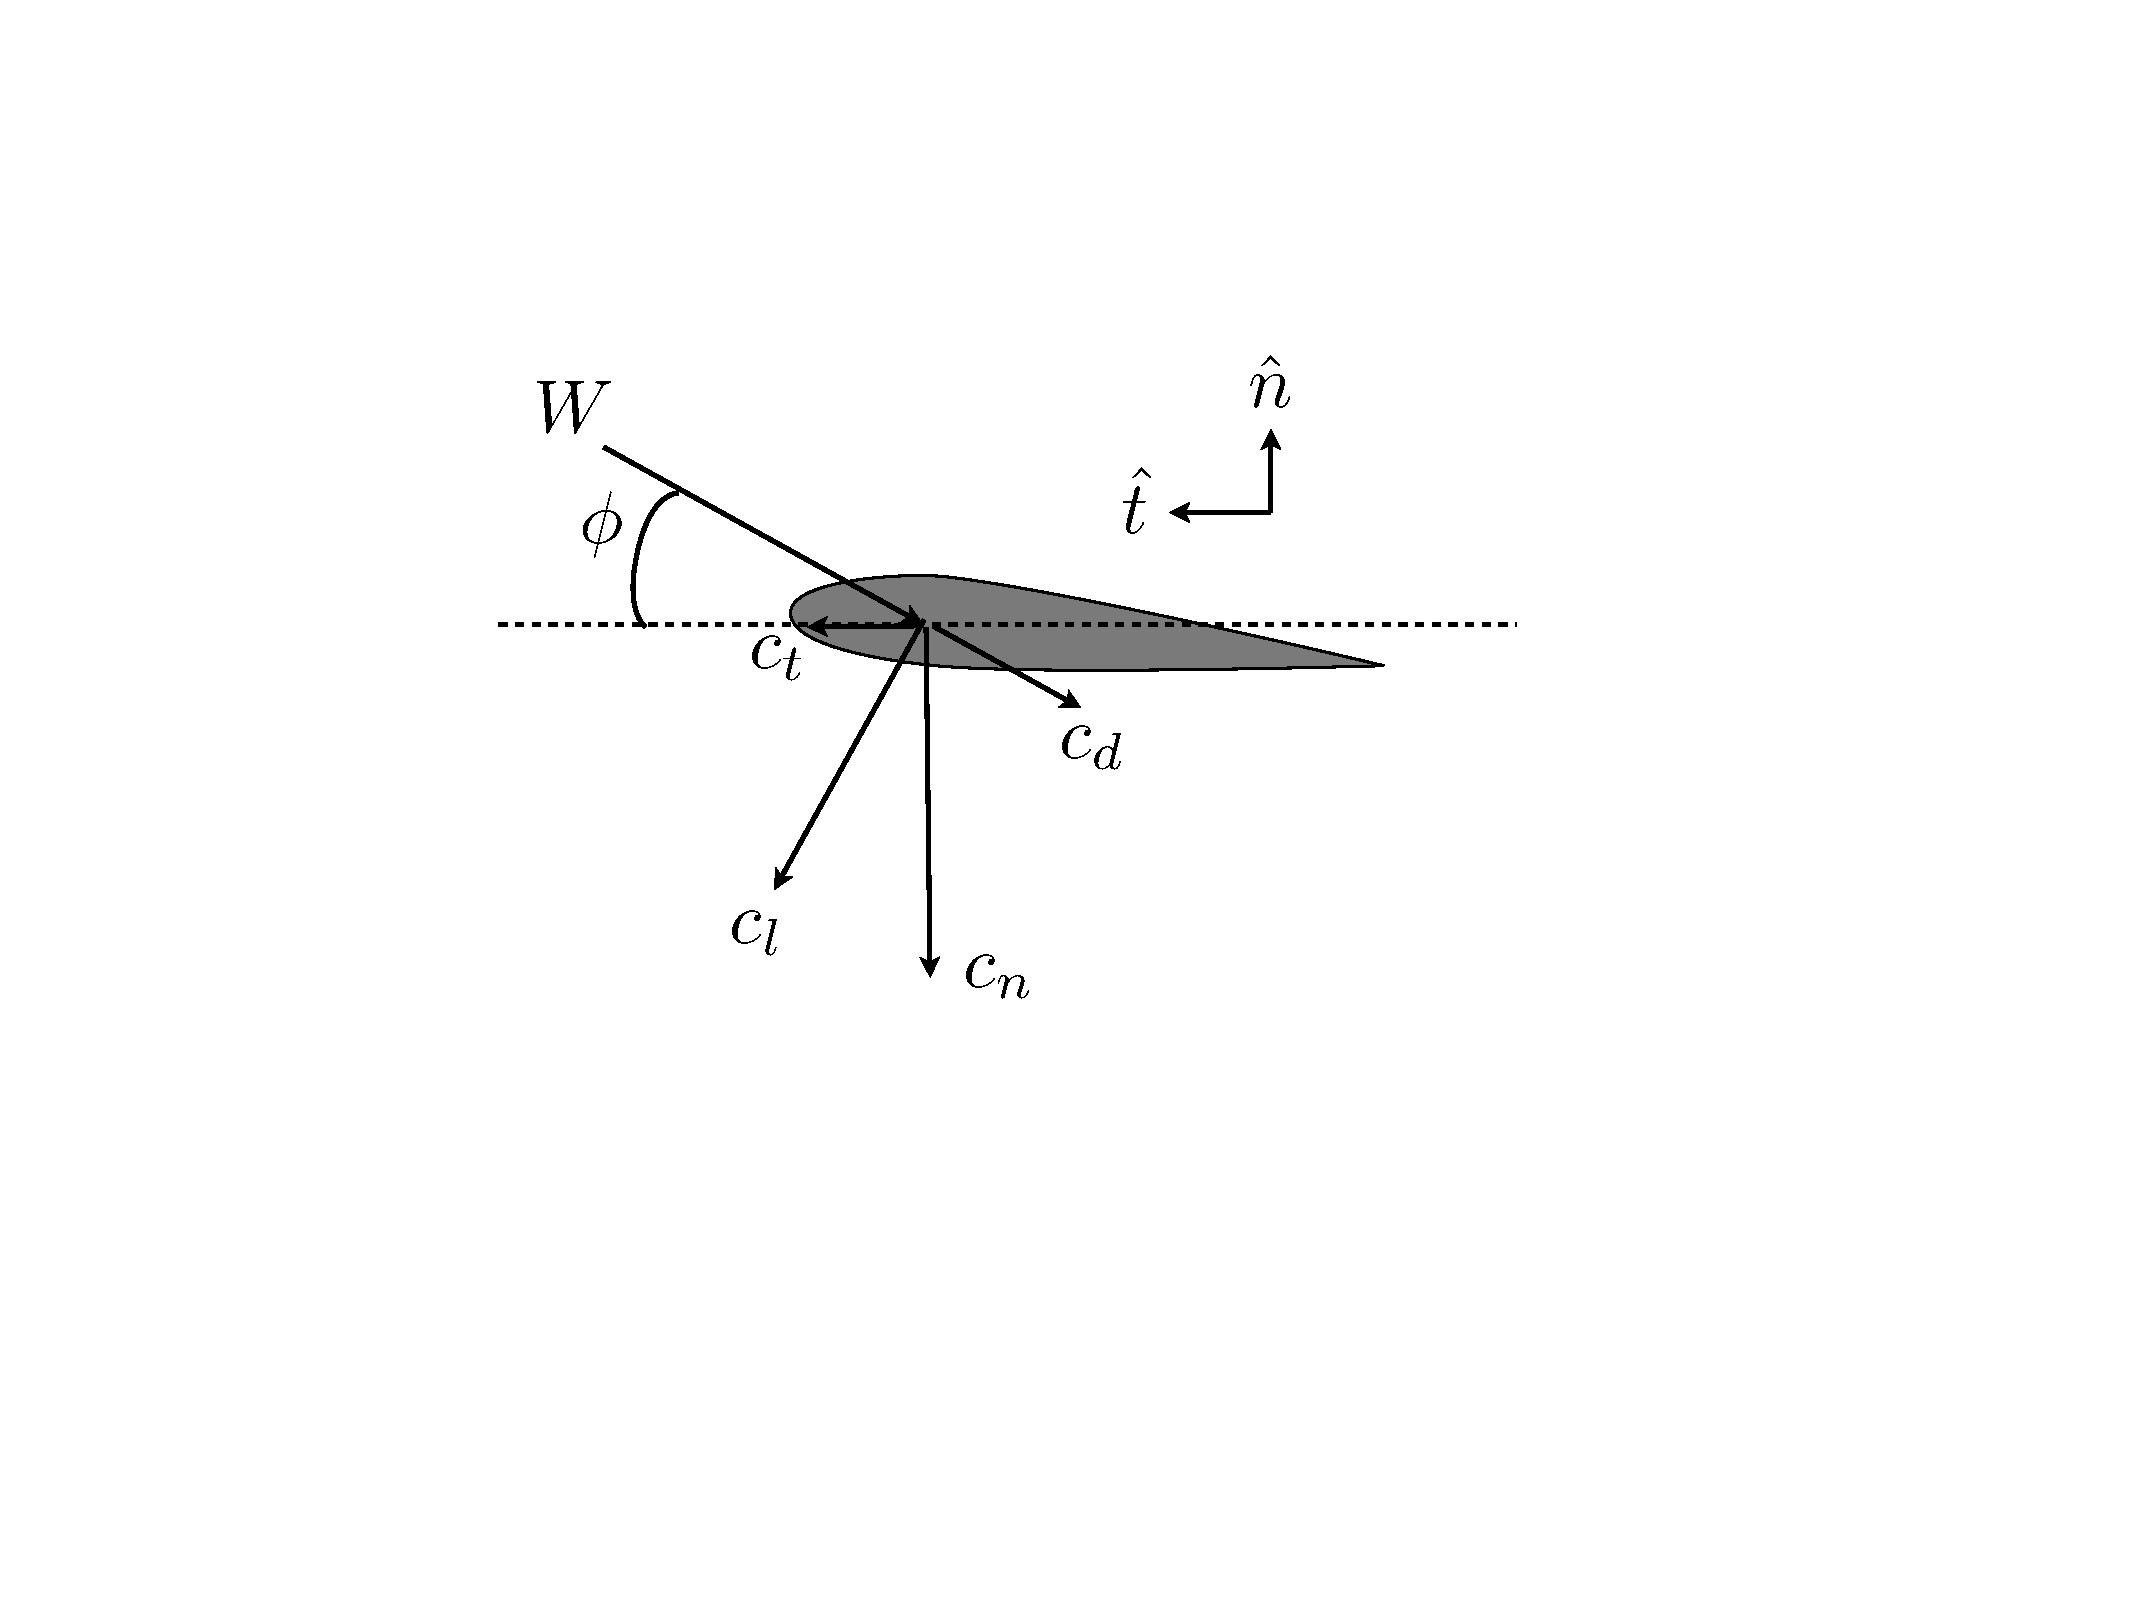
\includegraphics[width=3in]{images/cn}
\caption{Definition of normal and tangential force coefficients.}
\label{fig:cn}
\end{center}
\end{figure}

To expand these force coefficients into a distributed load, we need to compute the area of the blade element for a given length $dz$ in the z-direction.  From \Cref{fig:dl} we see that this area is
\begin{equation}
 da = c\ ds = c \frac{dz}{\cos\delta}
\end{equation}
Because sweeping is a shearing operation it does not increase the area of the blade element.  Using this area the force per unit length in the airfoil plane is
\begin{equation}
  F^\prime = \frac{\rho W^2 c}{2 \cos\delta} (-c_n \hat{n} + c_t\hat{t})
\end{equation}
where the negative sign results from our definition of $c_n$ being opposite to that of $\hat{n}$.  We can now rotate this force back to the cylinder plane
\begin{equation}
  F^\prime = \frac{\rho W^2 c}{2 \cos\delta} (-c_n \cos\delta \hat{r} - c_n\sin\delta \hat{z} + c_t\hat{t})
\end{equation}
The three force components (radial, tangential, vertial) per unit length in the z-direction can be expressed as
\begin{equation}
\begin{aligned}
  R^\prime &= -c_n \frac{1}{2} \rho W^2 c \\
  T^\prime &= c_t \frac{1}{2}\rho W^2 \frac{c}{\cos\delta } \\
  Z^\prime &= -c_n\frac{1}{2}\rho W^2 c \tan\delta
  \label{eq:forces}
\end{aligned}
\end{equation}

\begin{figure}[htbp]
\begin{center}
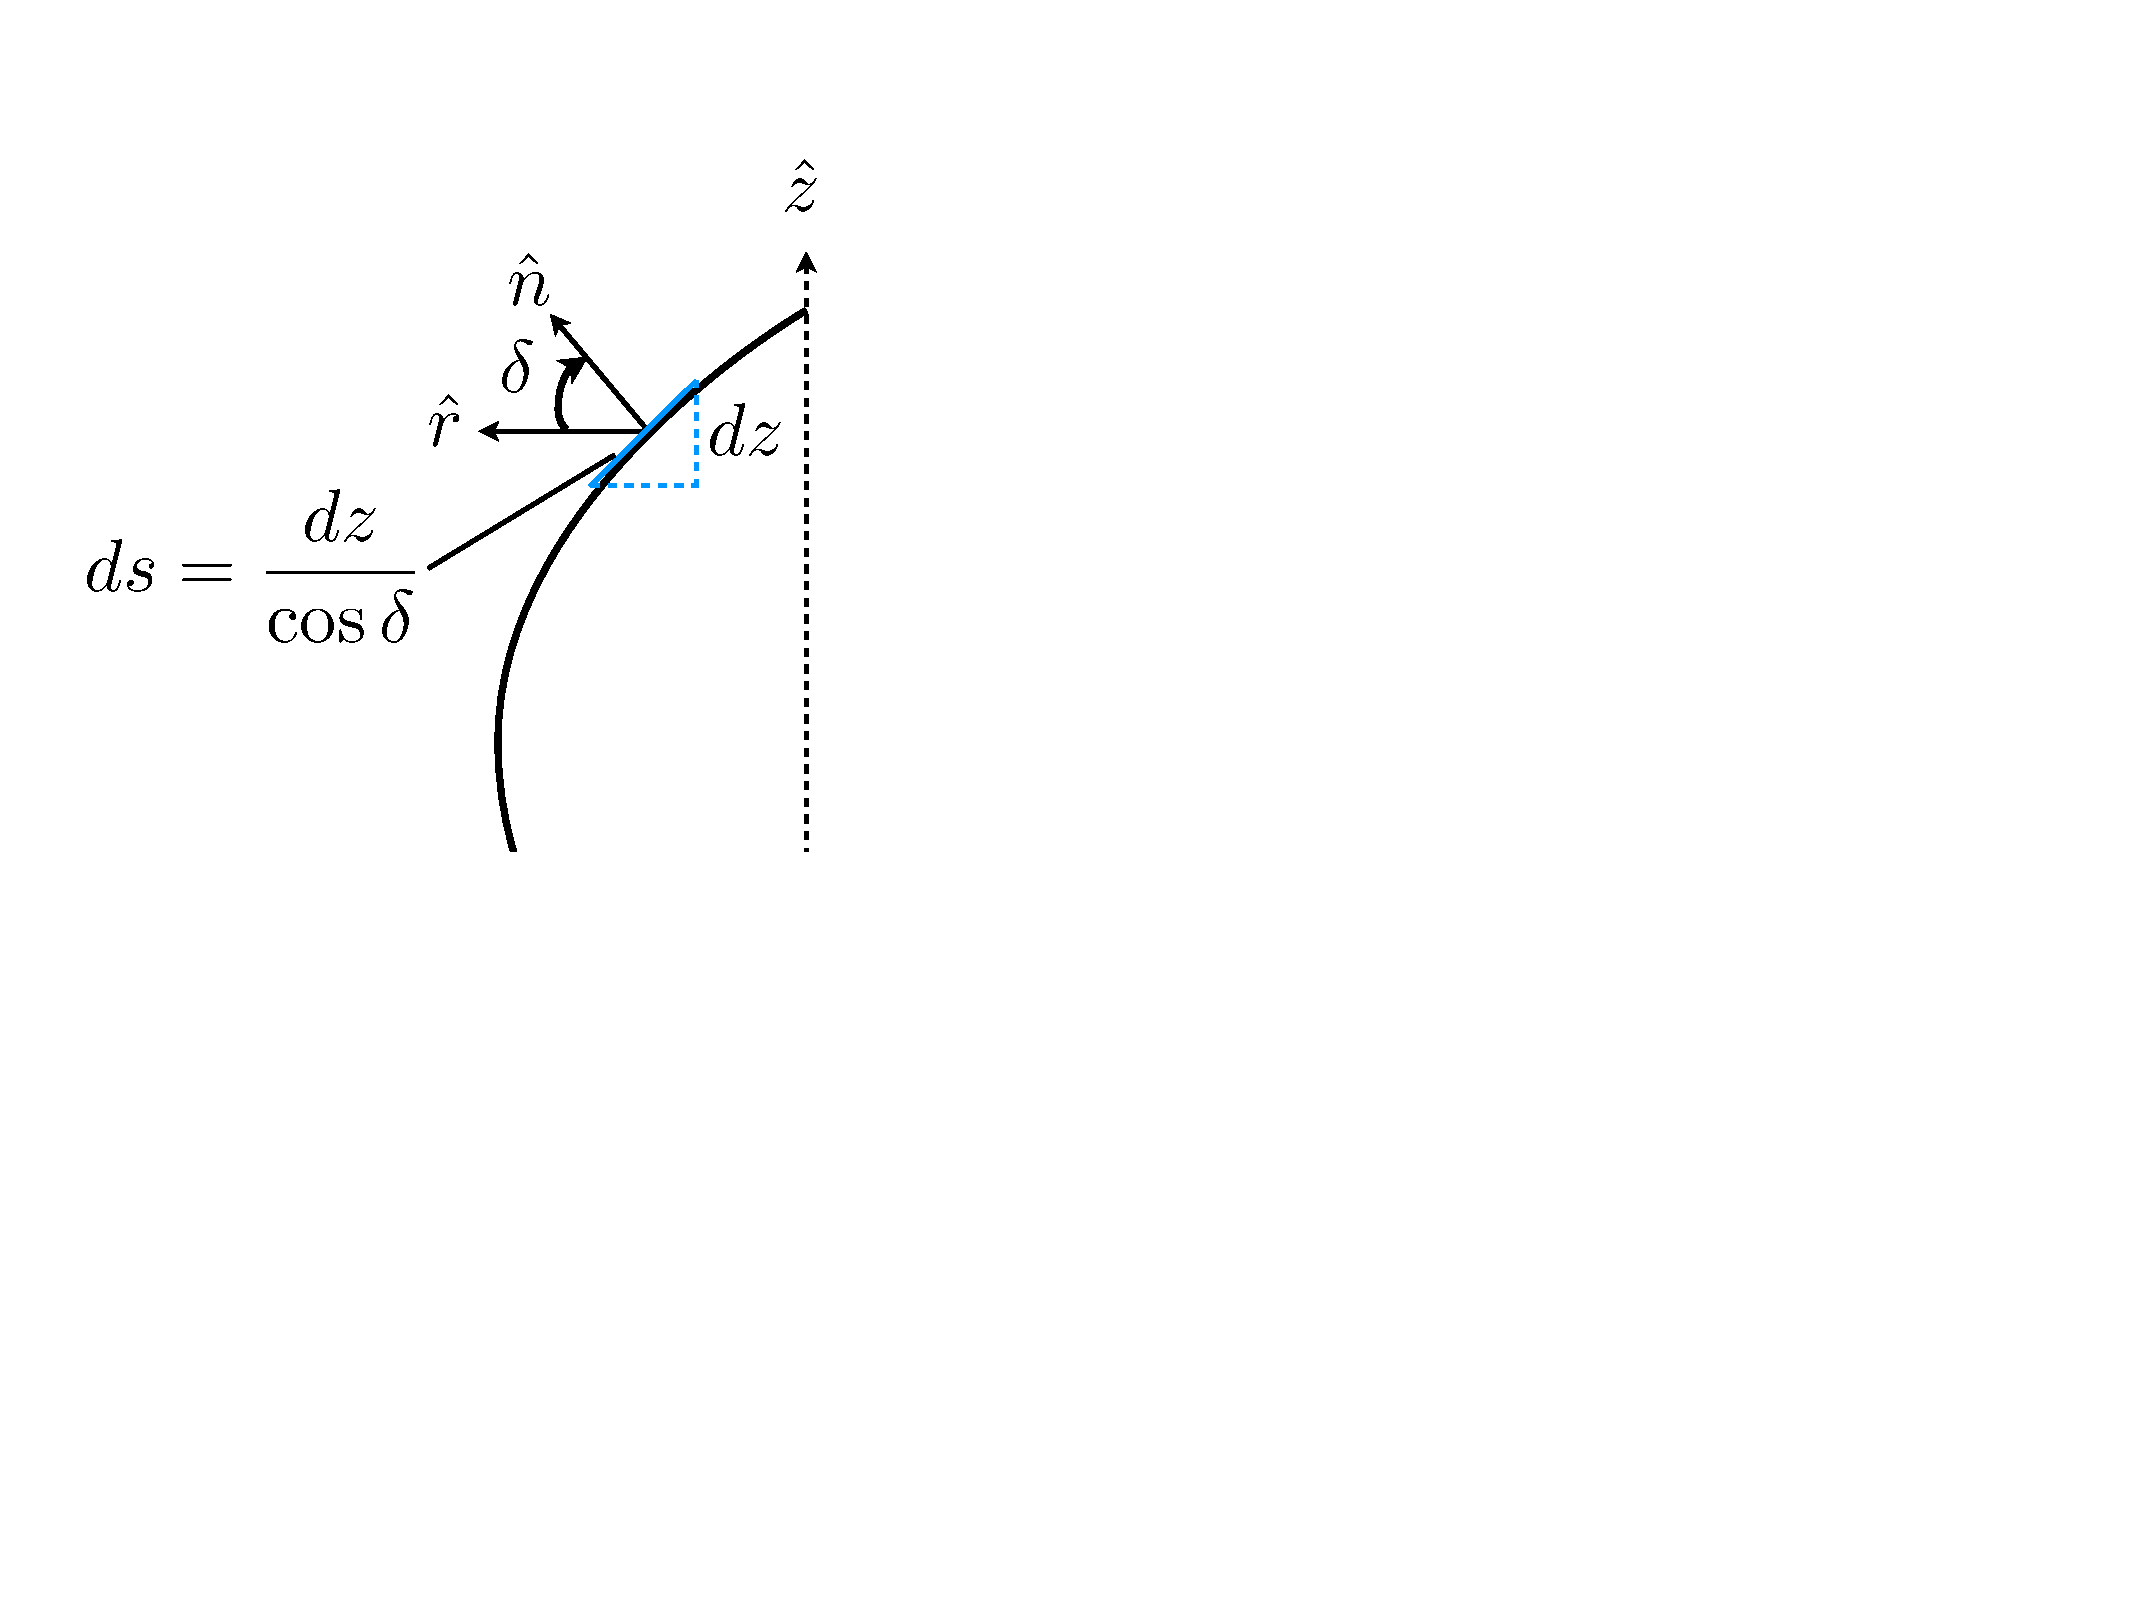
\includegraphics[width=2in]{images/dl}
\caption{Cross-sectional length of blade segment for small changes in height.  Blade curvature increases the area of the blade element for unit height, but sweep has no effect on the blade element area as it is a shearing operation.}
\label{fig:dl}
\end{center}
\end{figure}


For purposes of the blade element method we are interested in the force in the x-direction
\begin{equation}
\begin{aligned}
  X^\prime &= -R^\prime \sin\theta - T^\prime \cos\theta \\
  &= \frac{1}{2} \rho W^2 c\ (c_n \sin\theta - c_t \frac{\cos \theta}{\cos\delta})
  \label{eq:xprime}
\end{aligned}
\end{equation}

This is an instantaneous value, but computing an azimuthal average across the front face of the stream tube results in
\begin{equation}
\begin{aligned}
  X^\prime_{streamtube} &= B \frac{\Delta \theta}{2\pi} X^\prime\\
  &= B \frac{\Delta \theta}{4\pi} \rho W^2 c\ (c_n \sin\theta - c_t \frac{\cos \theta}{\cos\delta})
\end{aligned}
\end{equation}
The total force generated by the streamtube is $X^\prime_{streamtube} \Delta z$.  Normalizing this force using the same area used in the momentum method (Equation \eqref{eq:deltaA}) results in the following definition for the thrust coefficient from blade element theory
\begin{equation}
  C_T =  \frac{B c}{2 \pi r} \left(\frac{W}{V_\infty}\right)^2   (c_n \sin\theta - c_t \frac{\cos \theta}{\cos\delta}) \frac{1}{|\sin\theta| }
  \label{eq:ctbem}
\end{equation}

\subsection{Solution Procedure}

The solution procedure for a single streamtube consists of solving two sequential one-dimensional root finding problems.  The steps are

\begin{enumerate}
\item Start with a guess for $a$
\item Compute reduced velocity \eqref{eq:V} (or \eqref{eq:Vprime} for second surface of actuator cylinder)
\item Compute angle of attack, Reynolds number, and inflow angle \eqref{eq:alpha}
\item Compute airfoil section lift and drag
\item Rotate to get normal and tangential force coefficients  \eqref{eq:cn}
\item Compute the thrust coefficient from blade element momentum theory \eqref{eq:ctbem}
\item Compute the thrust coefficient from momentum theory \eqref{eq:ctmom} or \eqref{eq:ctglauert}
\item Compute the residual $f(a) = C_T(a)_{momentum} - C_T(a)_{bem}$
\end{enumerate}

In practice the root is best solved with a bracketing method such as Brent's method.  Once the value for $a$ is found for the first surface, the induction factor $a^\prime$ must be found for the back surface.  The solution procedure is the same, except $V_e = (1-2a)V_\infty$ is used in place of $V_\infty$ and of course the value for $\theta$ is changed.  After the induction factor has been solved at a given location, the corresponding forces can be computed from \eqref{eq:forces}.


\section{Actuator Cylinder Theory}
As discussed in \Cref{sec:dmst}, double multiple streamtube theory, is a useful but a somewhat forced application of actuator disk theory to a VAWT.  Ideally, one would like to model the actual swept surface of the blades, which leads to actuator cylinder theory.  The theory begins with the two-dimensional, steady, incompressible, Euler equations (continuity and momentum)
\begin{equation}
\frac{\partial u}{\partial x} + \frac{\partial v}{\partial y} = 0
\label{eq:continuity}
\end{equation}
\begin{equation}
\begin{aligned}
\frac{\partial u u}{\partial x} + \frac{\partial u v}{\partial y} &= \frac{1}{\rho}\left( -\frac{\partial p}{\partial x} + f_x\right)\\
\frac{\partial u v}{\partial x} + \frac{\partial v v}{\partial y} &= \frac{1}{\rho}\left(-\frac{\partial p}{\partial y} + f_y\right)
\label{eq:euler}
\end{aligned}
\end{equation}
where the $f_i$ terms are body forces per unit volume (in this case forces produces by the VAWT).  Expanding the derivatives in the momentum equations using the chain rule and canceling terms using the continuity equation leads to
\begin{equation}
\begin{aligned}
u \frac{\partial u}{\partial x} + v \frac{\partial u}{\partial y} &= \frac{1}{\rho}\left( -\frac{\partial p}{\partial x} + f_x\right) \\
u \frac{\partial v}{\partial x} + v \frac{\partial v}{\partial y} &= \frac{1}{\rho}\left( -\frac{\partial p}{\partial y} + f_y\right)
\label{eq:euler1}
\end{aligned}
\end{equation}
Since the freestream is in the x-direction we can write the velocities as a sum of the freestream velocity and a perturbation velocity (similarly with pressure)
\[ u = U_\infty + u^\prime \]
\[ v = v^\prime \]
\[ p = p_\infty + p^\prime \]
Substituting these into equation \eqref{eq:euler1} leads to
\begin{equation}
\begin{aligned}
U_\infty \frac{\partial u^\prime}{\partial x} + u^\prime \frac{\partial u^\prime}{\partial x} + v^\prime \frac{\partial u^\prime}{\partial y} &= \frac{1}{\rho}\left( -\frac{\partial p^\prime}{\partial x} + f_x\right) \\
U_\infty \frac{\partial v^\prime}{\partial x} + u^\prime \frac{\partial v^\prime}{\partial x} + v^\prime \frac{\partial v^\prime}{\partial y} &= \frac{1}{\rho}\left( -\frac{\partial p^\prime}{\partial y} + f_y\right)
\end{aligned}
\end{equation}
We can now make these equations nondimensional by multiplying through by $R/U_\infty^2$
\begin{equation}
\begin{aligned}
\frac{\partial u^*}{\partial x^*} + u^* \frac{\partial u^*}{\partial x} + v^* \frac{\partial u^*}{\partial y^*} &= -\frac{\partial p^*}{\partial x^*} + f_x^*\\
\frac{\partial v^*}{\partial x^*} + u^* \frac{\partial v^*}{\partial x^*} + v^* \frac{\partial v^*}{\partial y^*} &= -\frac{\partial p^*}{\partial y^*} + f_y^*
\label{eq:normalized}
\end{aligned}
\end{equation}
where $x^* = x/R$, $y^* = y/R$, $u^* = u^\prime/U_\infty$, $v^* = v^\prime/U_\infty$, $p^* = p^\prime/(\rho U_\infty^2)$, and $f^* = f R / (\rho U_\infty^2)$.  For simplicity the exponent $^*$ will be dropped in the following equations, with the understanding that the values are properly normalized.  We can arrange these equations into a sum of a linear and nonlinear term.
\begin{equation}
\begin{aligned}
\frac{\partial u}{\partial x}  &= -\frac{\partial p}{\partial x} +f_x +  g_x\\
\frac{\partial v}{\partial x} &= -\frac{\partial p}{\partial y} + f_y + g_y
\label{eq:euler2}
\end{aligned}
\end{equation}
where the nonlinear terms are given by
\begin{equation}
\begin{aligned}
g_x &= -u \frac{\partial u}{\partial x} - v \frac{\partial u}{\partial y}\\
g_y &= -u \frac{\partial v}{\partial x} - v \frac{\partial v}{\partial y}
\end{aligned}
\end{equation}
If we differentiate the first equation in \eqref{eq:euler2} by x and the second equation by y, add them together, and cancel terms using continuity \eqref{eq:continuity} the result is
\begin{equation}
\frac{\partial^2 p}{\partial x^2} + \frac{\partial^2 p}{\partial y^2} = \frac{\partial f_x}{\partial x} + \frac{\partial f_y}{\partial y} + \frac{\partial g_x}{\partial x} + \frac{\partial g_y}{\partial y}
\end{equation}
If we ignore the nonlinear terms ($g_x$ and $g_y$) then we have a Poisson-type equation
\begin{equation}
\nabla^2 p = \nabla \cdot f
\end{equation}
This equation, combined with the boundary condition that the perturbation pressure goes to zero at infinity, yields the solution
\begin{equation}
p_{linear} = \frac{1}{2\pi}\int\int \frac{f_x(x-\xi) + f_y(y-\eta)}{(x-\xi)^2 + (y-\eta)^2} d\xi d\eta
\end{equation}
the volume forces are zero everywhere except along the cylinder where $\xi = -\sin\theta$ and $\eta = \cos\theta$, thus
\begin{equation}
p_{linear} = \frac{1}{2\pi}\int\limits_0^{2\pi} \frac{f_x(x+\sin\theta) + f_y(y-\cos\theta)}{(x+\sin\theta)^2 + (y-\cos\theta)^2} d\theta
\label{eq:pfxfy}
\end{equation}

The volume forces produced by the VAWT are modeled as acting along an infinitesimally small radial distance, and in a direction normal to the surface of the cylinder (the tangential component is much smaller than the normal force and can be reasonably neglected in this analysis).  The radial volume force is
\begin{equation}
   f_r(\theta) = \frac{F_r^\prime}{r \Delta\theta \Delta r} \frac{R}{\rho U_\infty^2}
\end{equation}
where $F_r^\prime$ is the radial force per unit length, $r \Delta\theta \Delta r$ is the in-plane area across which the force acts (Figure \ref{fig:deltaA}), and the last term comes from the normalization in \eqref{eq:normalized}.

\begin{figure}[htbp]
\begin{center}
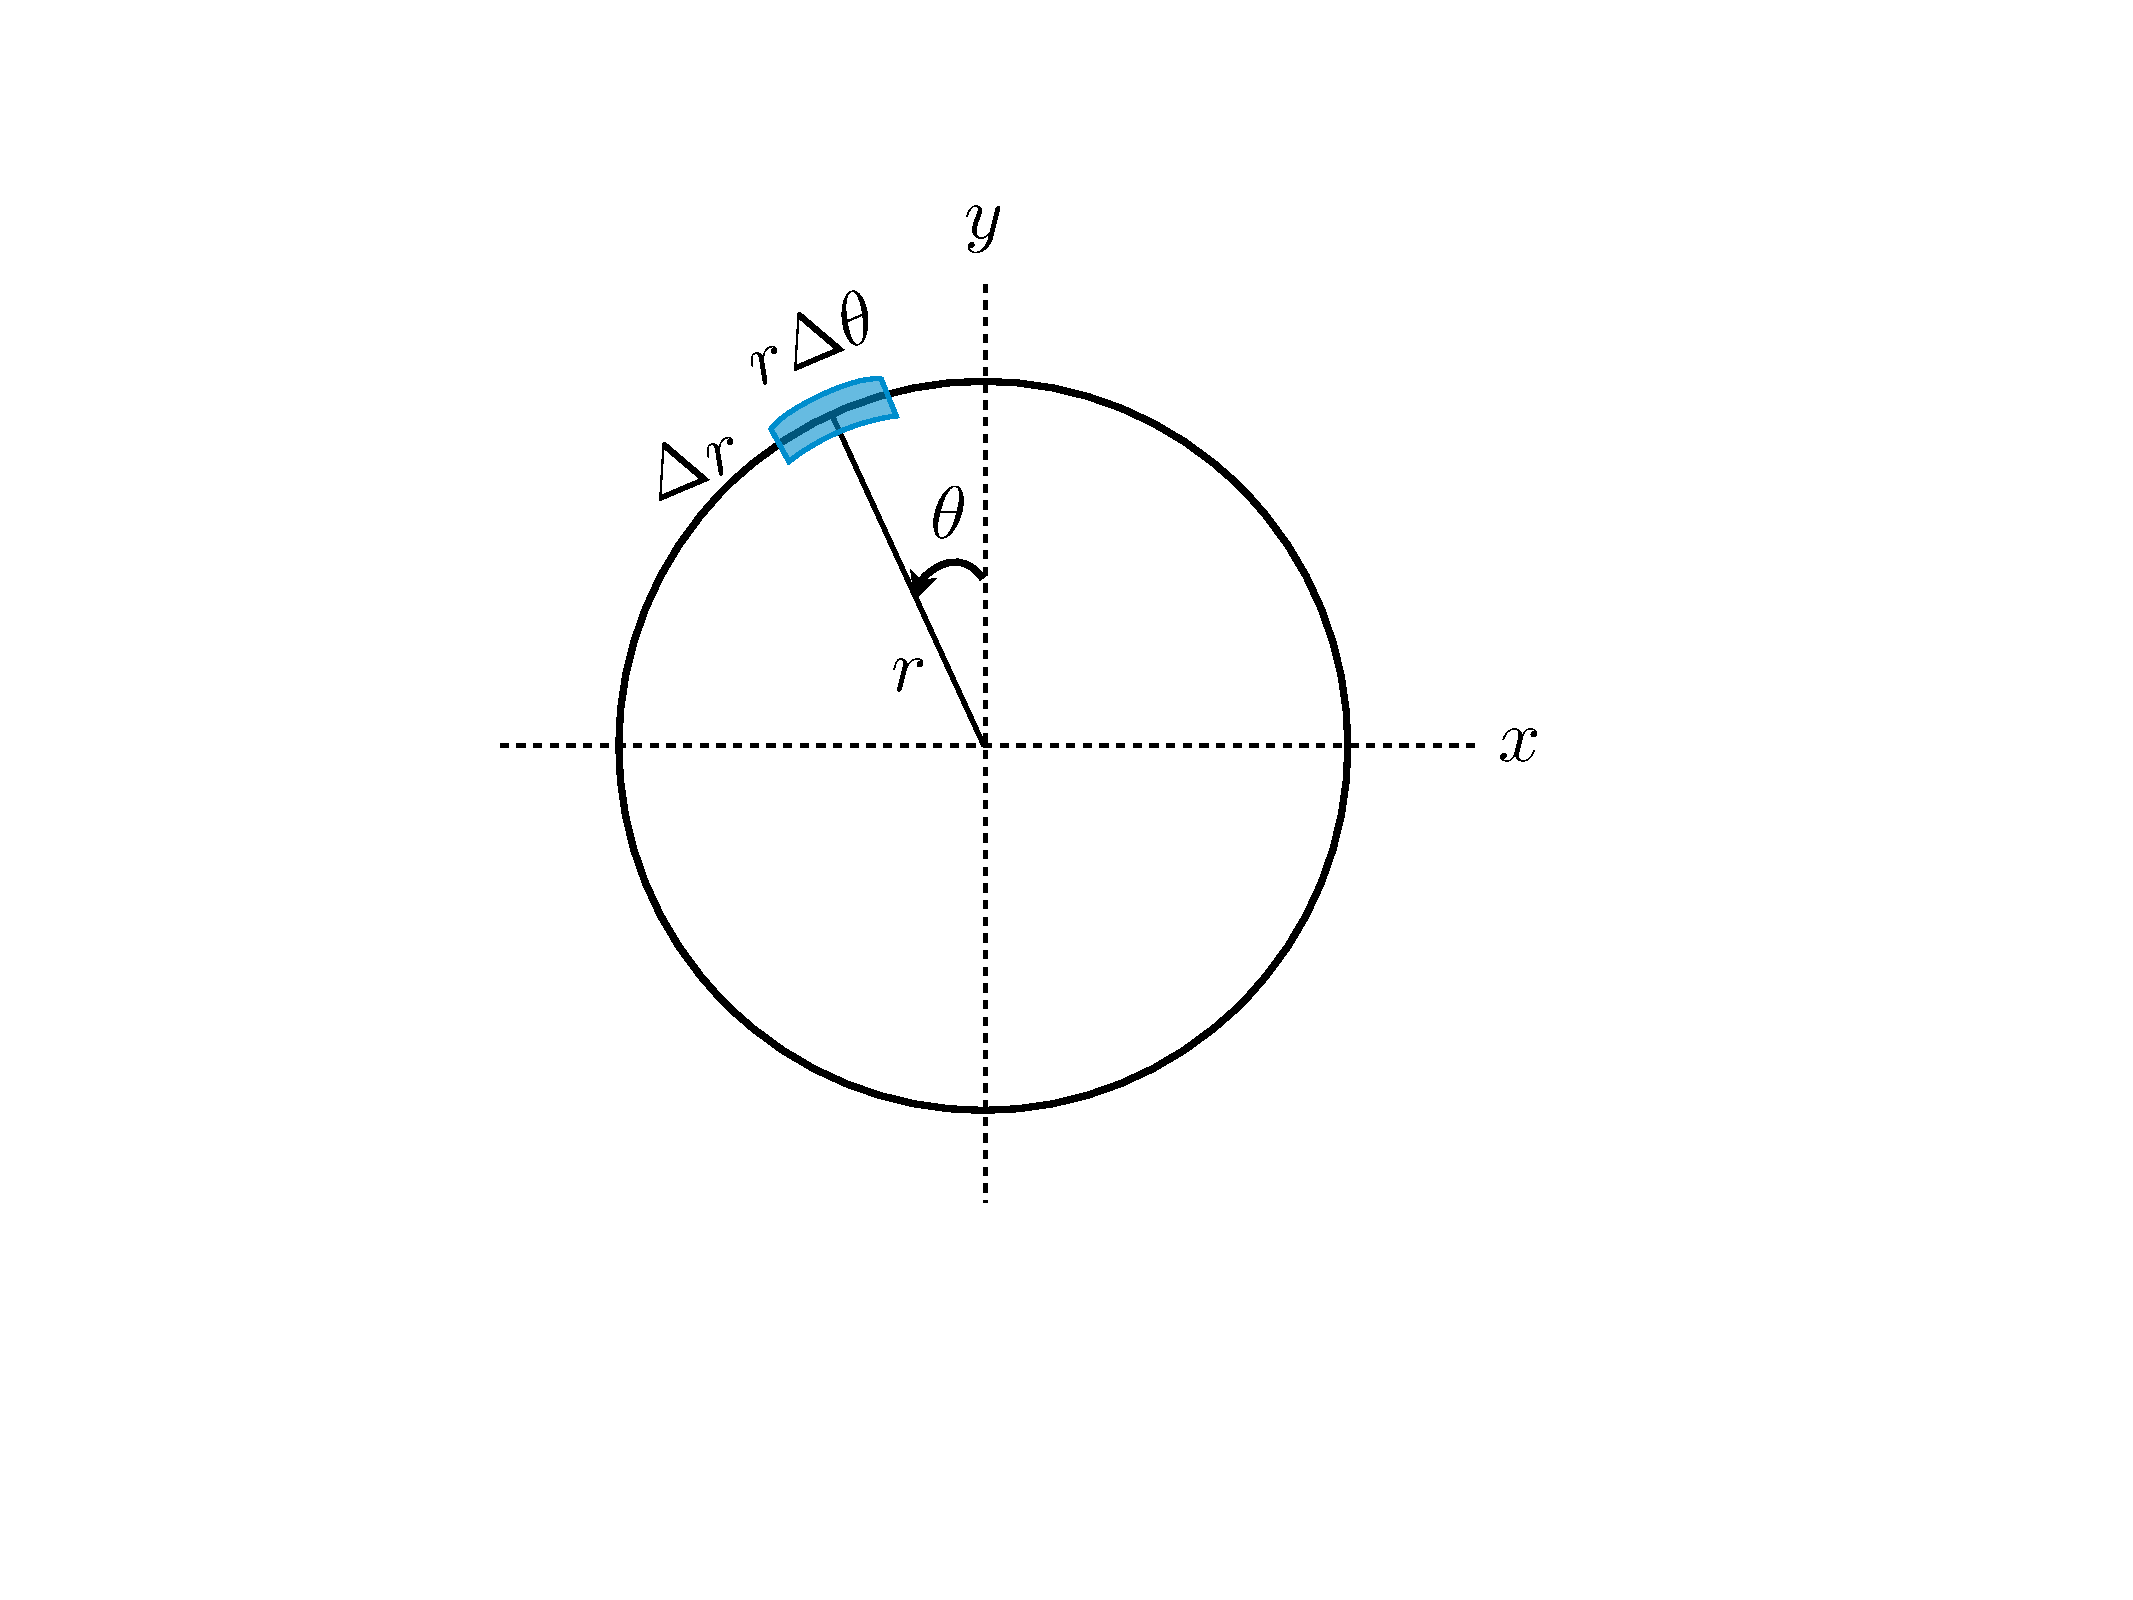
\includegraphics[width=2.5in]{images/deltaA}
\caption{In-plane area for volume force at a given azimuthal station.}
\label{fig:deltaA}
\end{center}
\end{figure}

Because the force acts across an infestesimal small radial distance, the volume force acts as a pressure jump
\begin{equation}
  Q_r(\theta) = \lim_{\epsilon \rightarrow 0} \frac{1}{R} \int\limits_{r-\epsilon}^{r+\epsilon} f_r(\theta) dr = \lim_{\epsilon \rightarrow 0} \frac{1}{R} \int\limits_{r-\epsilon}^{r+\epsilon}\frac{F_r^\prime}{r \Delta\theta dr} \frac{R}{\rho U_\infty^2} dr = \frac{F_r^\prime}{r \Delta\theta} \frac{1}{\rho U_\infty^2}
  \label{eq:Qr}
\end{equation}
 the $1/R$ is necessary to be consistent with the normalization used in \eqref{eq:normalized}.

% The direction of the force produced by the VAWT on the fluid acts upstream (Figure ?).

We define the positive direction for this force $F_r(\theta)$ as positive radial outward (and thus positive radially inward for the loads the fluid produces on the VAWT).  Using this sign convention, $f_x = -Q_r(\theta)\sin\theta$ and $f_y = Q_r(\theta)\cos\theta$ and substituting into \eqref{eq:pfxfy} yields
\begin{equation}
p_{linear}(x, y) = \frac{1}{2\pi}\int\limits_0^{2\pi} Q_r(\theta) \frac{-(x+\sin\theta)\sin\theta + (y-\cos\theta)\cos\theta}{(x+\sin\theta)^2 + (y-\cos\theta)^2} d\theta
\end{equation}

Referring to equation \eqref{eq:euler2} we can find the velocities by integrating both sides of the equation from $-\infty$ to $x$ (using the fact that the perturbation pressure is zero at $-\infty$, and again ignoring nonlinear terms)
\begin{equation}
u(x, y) = -p_{linear}(x, y) + \int\limits_{-\infty}^x -Q_r(\theta) \sin\theta dx^\prime
\end{equation}
the last term is zero everywhere except across the surface of the cylinder.  As an example consider a point on the interior of the cylinder.  If we define $x_u$ and $x_d$ as the upstream and downstream points of integration along the cylinder (see Figure \ref{fig:slice}) then the integral reduces to
\begin{equation}
\int\limits_{-\infty}^x -Q_r(\theta) \sin\theta dx^\prime=  \int\limits_{x_u}^{x_d} -Q_r(\theta) \sin\theta dx^\prime
\end{equation}
However, the length of the integration path increases with $dx^\prime = dr^\prime/\sin\theta$ (Figure \ref{fig:slice}).  Because the radial distance will be made infinitesimally small we can consider the forces along the $x$ direction to be the same as long the $r$ direction.  The resulting integral is
\begin{equation}
\int\limits_{-\infty}^x -Q_r(\theta) \sin\theta dx^\prime=   \lim_{dr \rightarrow 0} \int\limits_{r_u}^{r_d} -Q_r(\theta) \ dr
\end{equation}

\begin{figure}[htbp]
\begin{center}
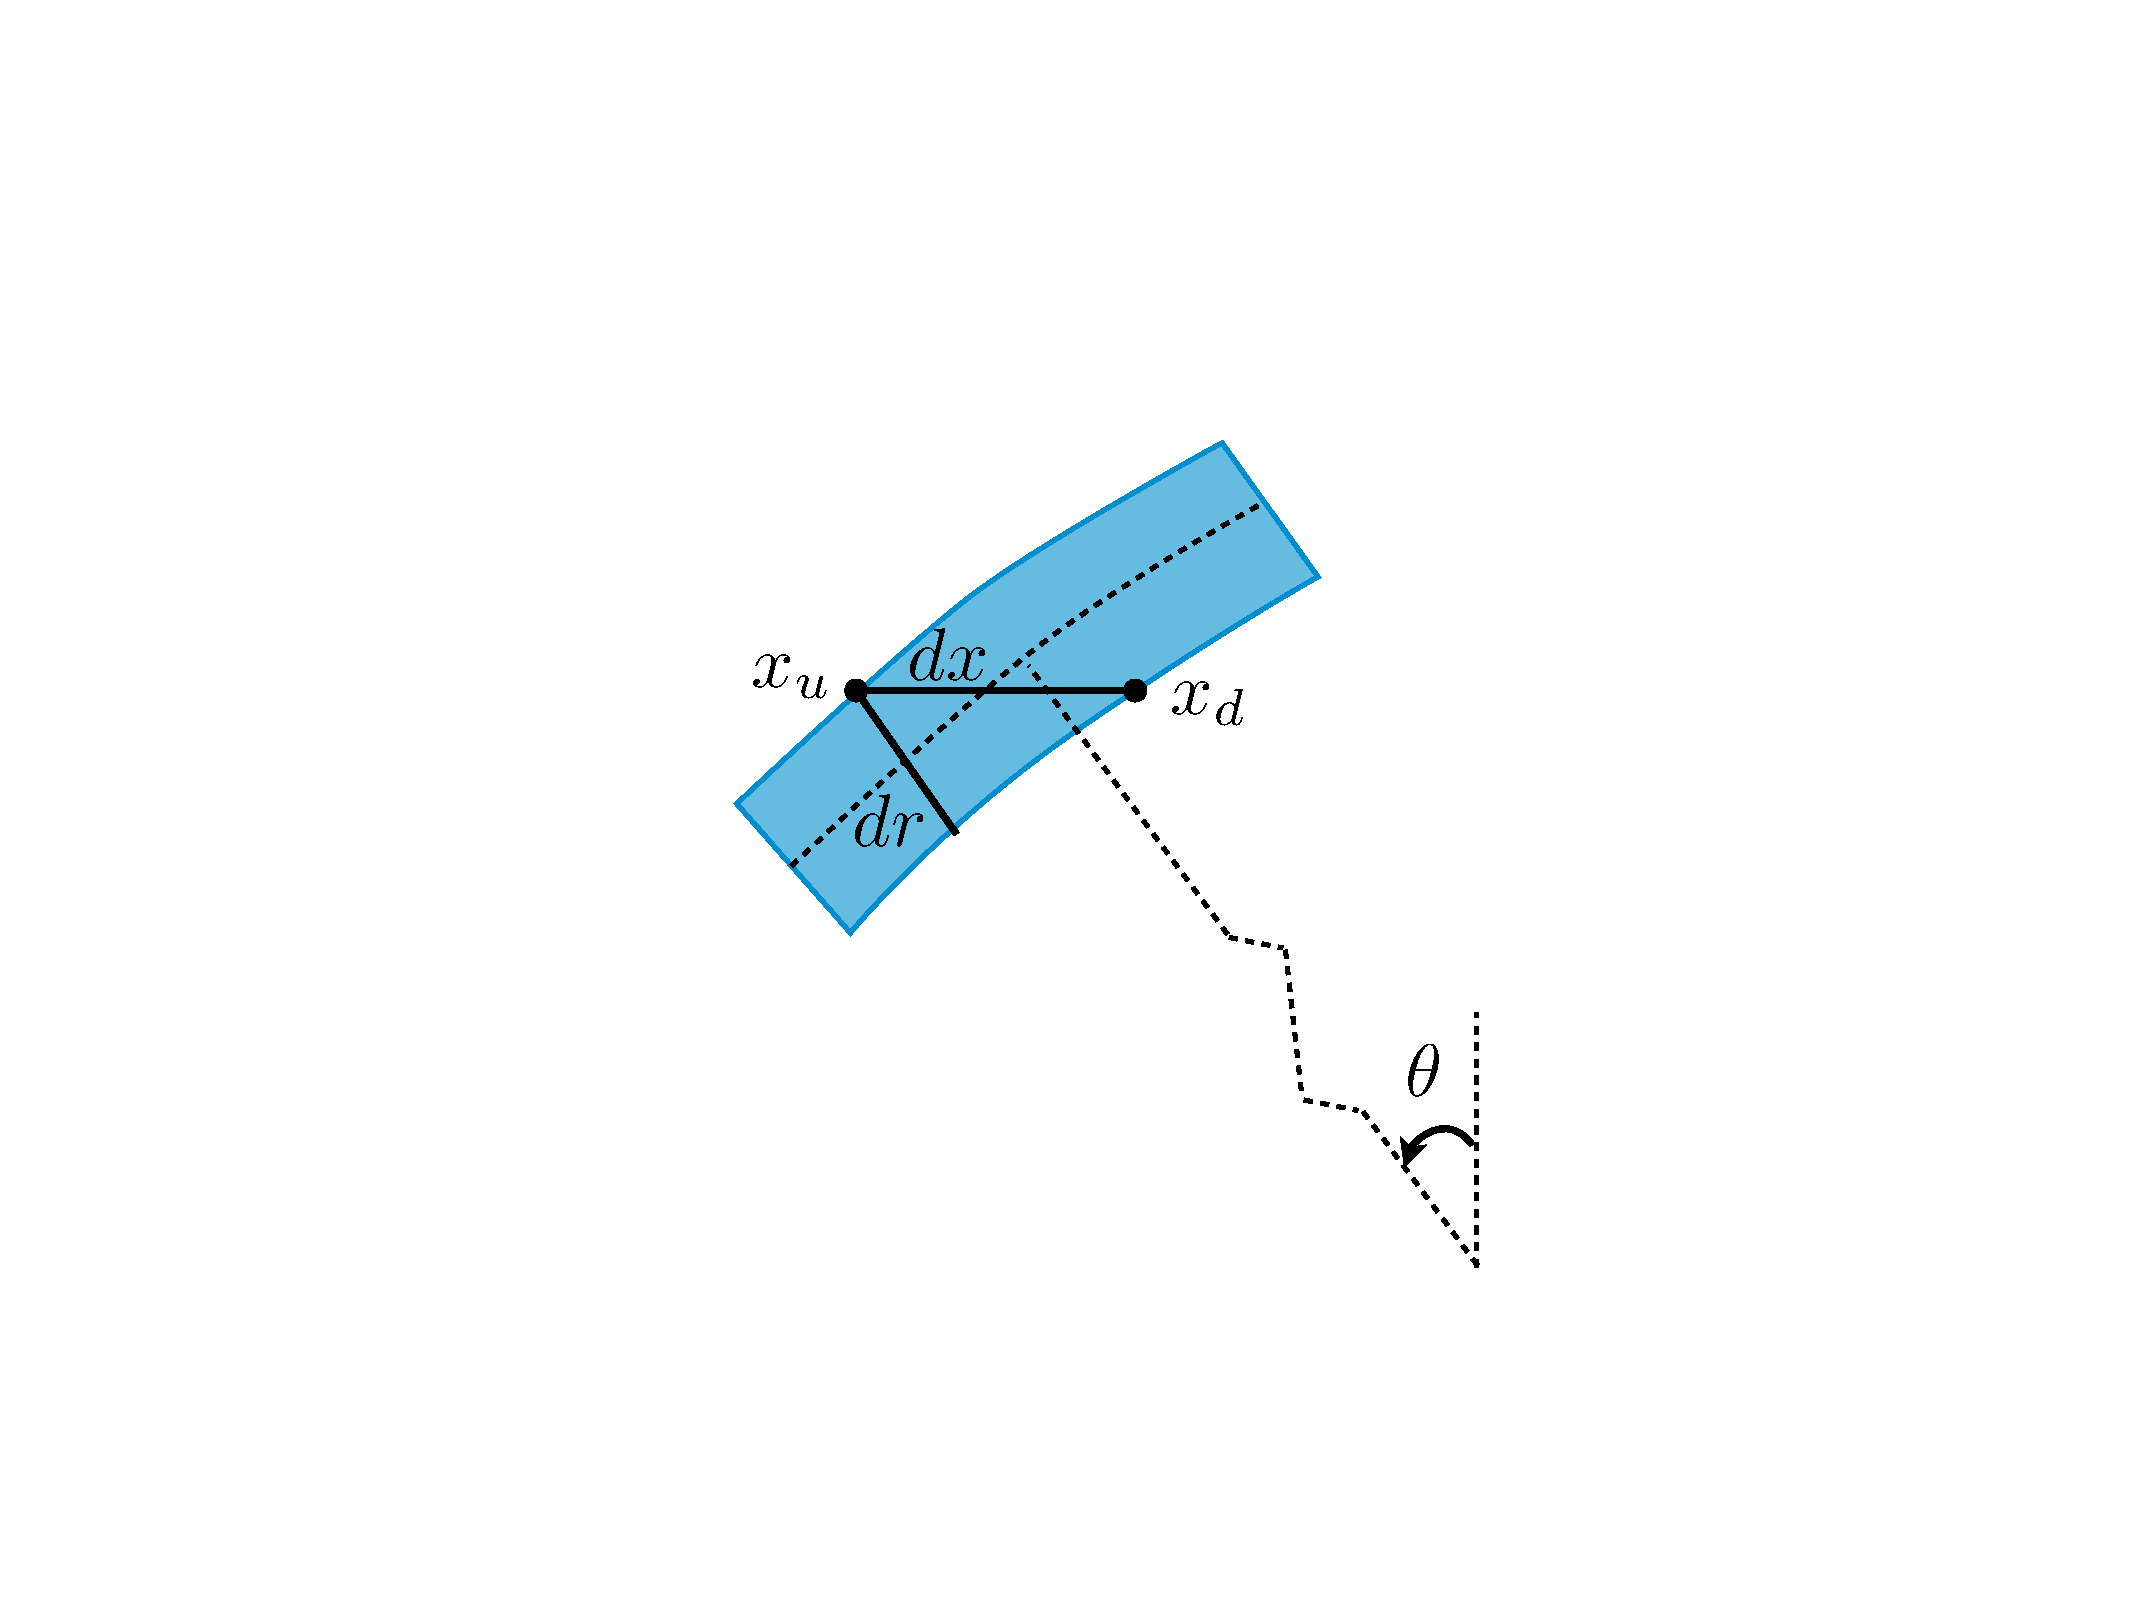
\includegraphics[width=2.5in]{images/slice}
\caption{A small section of actuator cylinder (exaggerated in size for clarity).  Integration occurs in x-direction.}
\label{fig:slice}
\end{center}
\end{figure}

In general, the value of the integral depends on whether the evaluation point is inside the cylinder, or behind it (i.e., $-1 < y^* >1 $).  If inside, $\theta = \cos^{-1} y$ (Figure \ref{fig:integration}) and the value of the integral is $-Q_r(\cos^{-1}y)$.  Behind the cylinder this term is also applicable plus an additional contribution from the downstream surface of the turbine where $\theta = -\cos^{-1} y$ and its contribution to the integral is $Q_r(-\cos^{-1}y) $
\begin{equation}
\begin{aligned}
u(x, y) =& -\frac{1}{2\pi}\int\limits_0^{2\pi} Q_r(\theta) \frac{-(x+\sin\theta)\sin\theta + (y-\cos\theta)\cos\theta}{(x+\sin\theta)^2 + (y-\cos\theta)^2} d\theta  \\
&- Q_r(\cos^{-1}y) \quad [\textrm{inside and wake}] \\
&+ Q_r(-\cos^{-1}y) \quad [\textrm{wake only}]
\label{eq:u}
\end{aligned}
\end{equation}
Inside the cylinder only the [inside and wake] term applies, and behind the cylinder both the [inside and wake] and [wake only] terms apply.

\begin{figure}[htbp]
\begin{center}
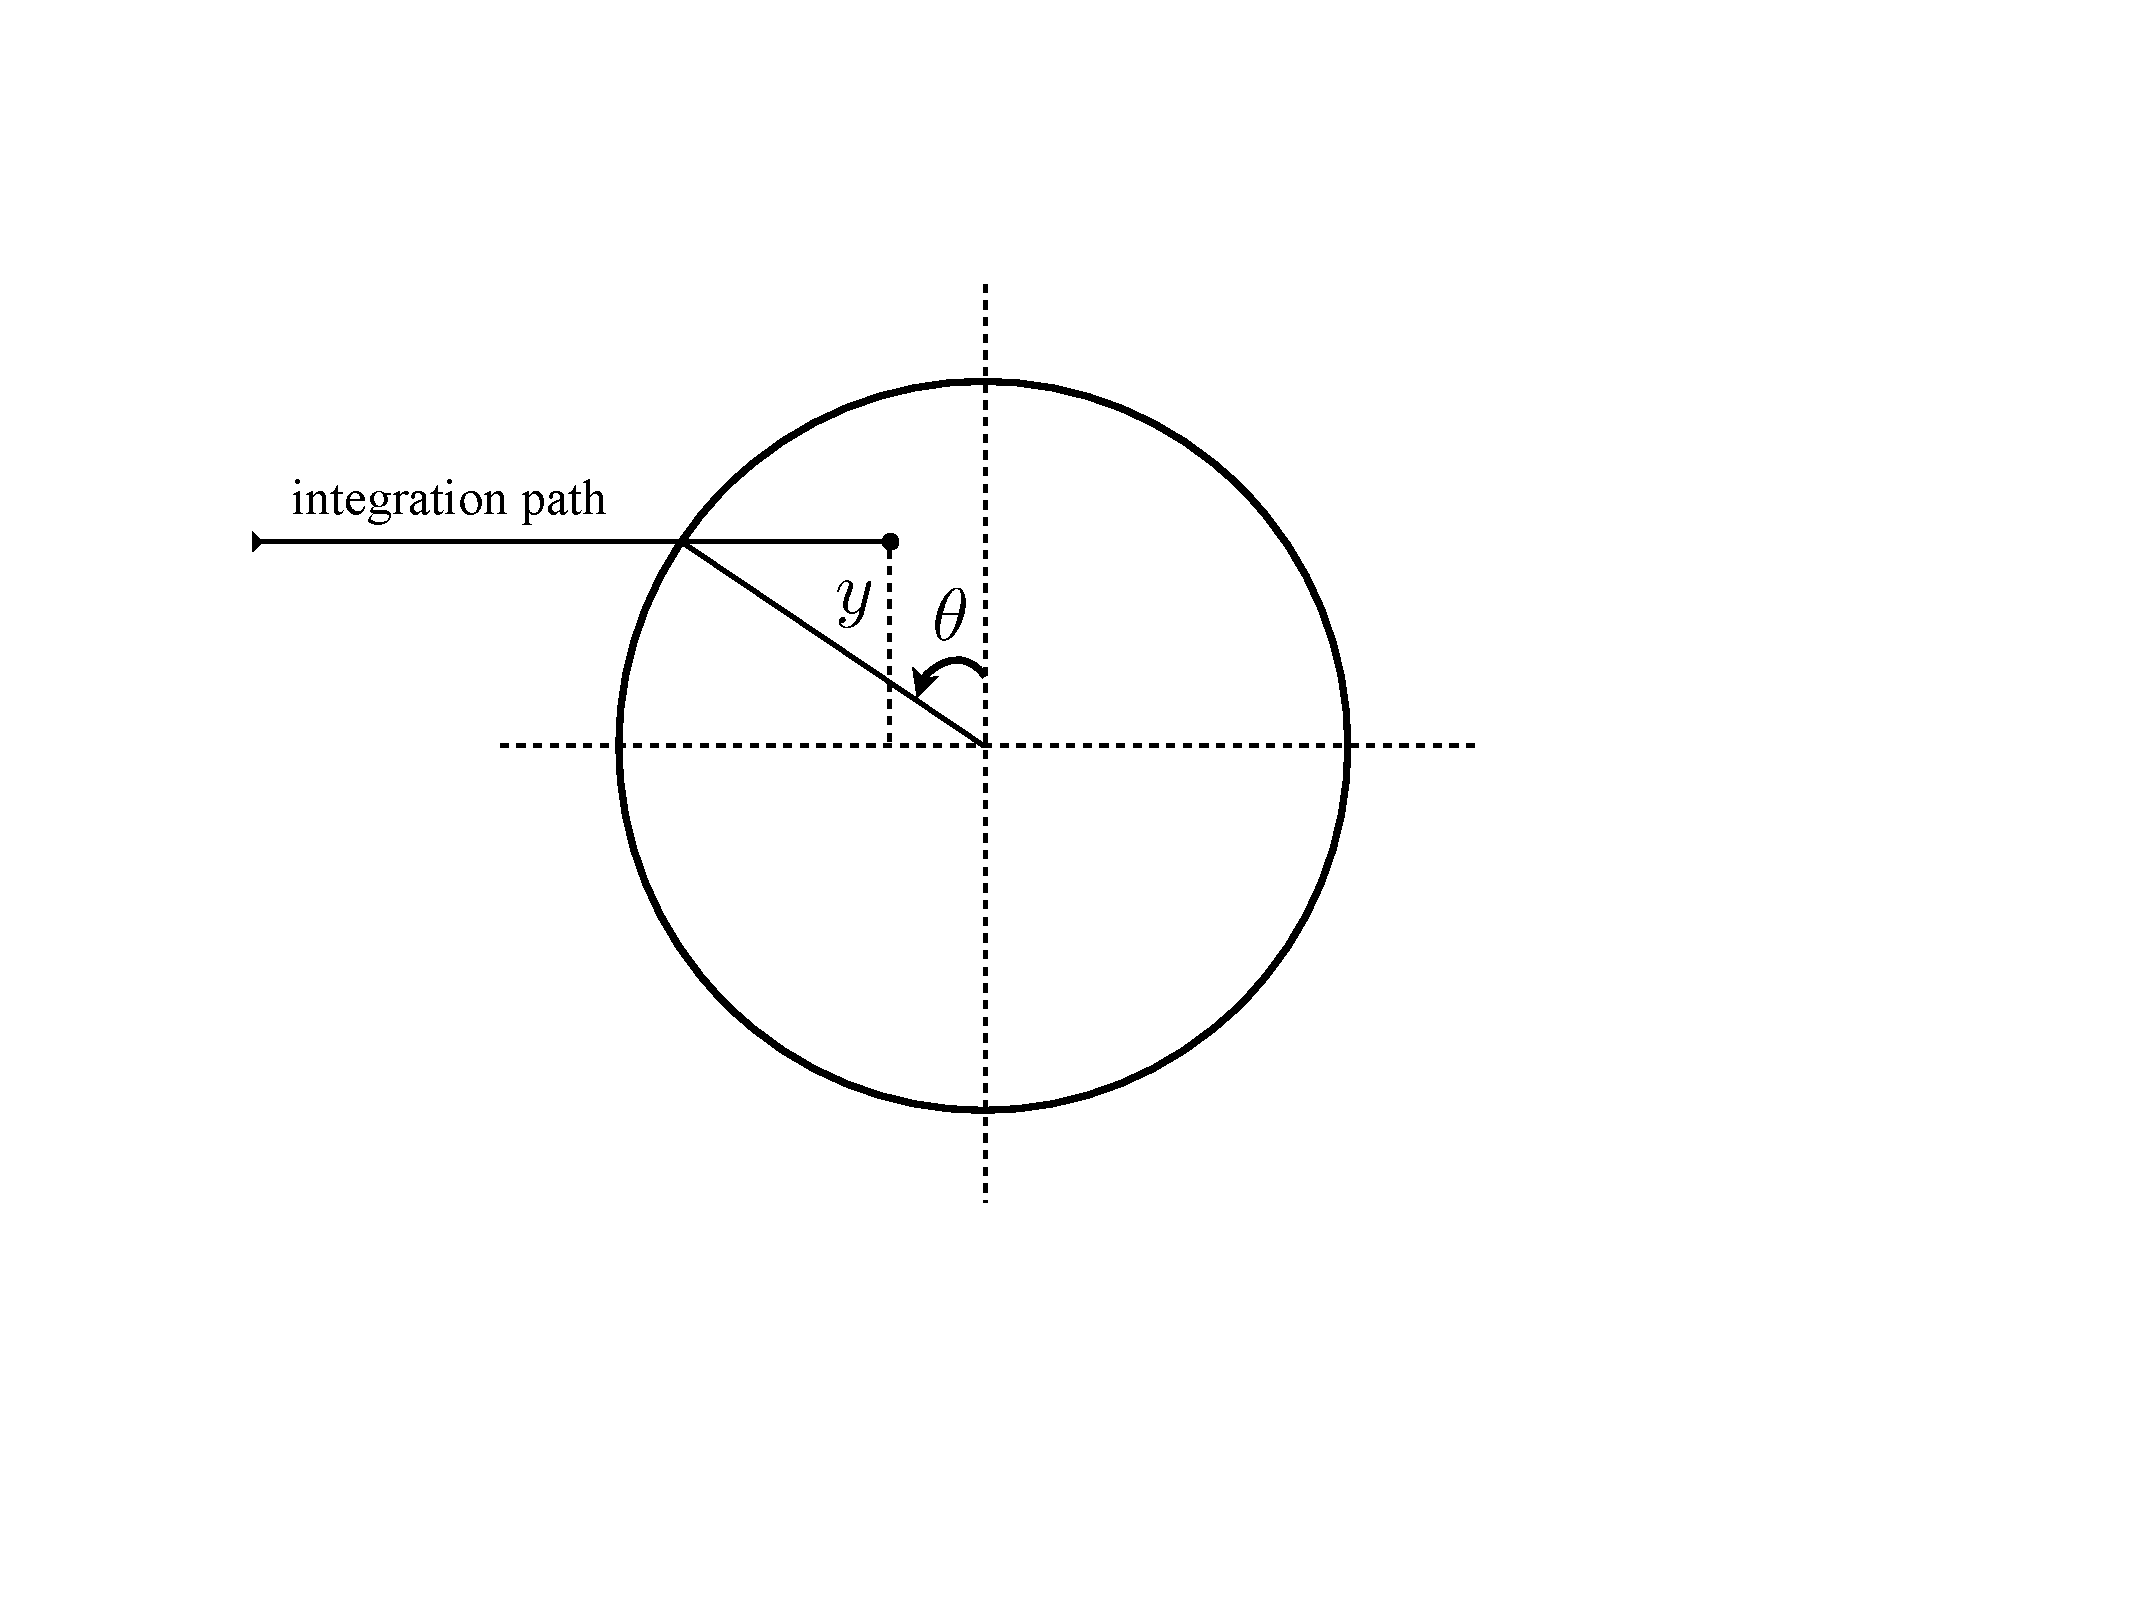
\includegraphics[width=3.5in]{images/integration}
\caption{Integration path for a point inside the cylinder.}
\label{fig:integration}
\end{center}
\end{figure}

In a similar manner we can find the velocities in the y-direction by integrating the second equation in \eqref{eq:euler2} from $-\infty$ to $x$ (again ignoring nonlinear terms)
\begin{equation}
  v(x, y) = \int\limits_{-\infty}^x-\frac{\partial p_{linear}}{\partial y} dx + \int\limits_{-\infty}^x f_y\ dx
\end{equation}
Performing the derivatives and integrating the vertical velocity results in
\begin{equation}
\begin{aligned}
v(x, y) =& -\frac{1}{2\pi}\int\limits_0^{2\pi} Q_r(\theta) \frac{-(x+\sin\theta)\cos\theta - (y-\cos\theta)\sin\theta}{(x+\sin\theta)^2 + (y-\cos\theta)^2} d\theta  \\
&+ c(y) + \int\limits_{-\infty}^x f_y\ dx
\end{aligned}
\end{equation}
where $c(y)$ is a constant of integration.  Similar to the previous case, the integral of the body force is only a function of $y$ and is only nonzero inside the cylinder or directly behind it.  Thus, both later terms are functions of $y$ only.  However, in the far-field the induced vertical velocity must go to zero.  Applying this boundary condition, both of these latter terms must be zero, and thus
\begin{equation}
v(x, y) = -\frac{1}{2\pi}\int\limits_0^{2\pi} Q_r(\theta) \frac{-(x+\sin\theta)\cos\theta - (y-\cos\theta)\sin\theta}{(x+\sin\theta)^2 + (y-\cos\theta)^2} d\theta
\label{eq:v}
\end{equation}

These two equations for the induced velocities (\eqref{eq:u} and \eqref{eq:v}) are applicable for any point in the plane, however for this application we are only interested in the induced velocity along the blade path.  To evaluate along the blade path, we discretize the description of the actuator cylinder into n sections as
\begin{equation}
\theta_i = (2i - 1) \frac{\pi}{n}  \quad \textrm{for } i = 1 \ldots n
\end{equation}
Furthermore, we assume piece-wise constant loading across each section.  The expression for the velocity predictions at the cylinder surface depend on whether we evaluate just upstream of the actuator disk or just downstream.  The end result is the same, as long as we are consistent.  In the following derivation we evaluate on the upstream surfaces for both halves of the actuator disk. The induced velocities along the cylinder are then
\begin{equation}
\begin{aligned}
u_i =& \frac{1}{2\pi} \sum\limits_j  {Q_r}_j  \int\limits_{\theta_j - \Delta\theta/2}^{\theta_j + \Delta\theta/2} \frac{(x_i+\sin\theta)\sin\theta - (y_i-\cos\theta)\cos\theta}{(x_i+\sin\theta)^2 + (y_i-\cos\theta)^2} d\theta  \\
&- {Q_r}_{(n+1-i)}\quad [i > n/2]
\end{aligned}
\end{equation}
\begin{equation}
v_i = \frac{1}{2\pi} \sum\limits_j  {Q_r}_j  \int\limits_{\theta_j - \Delta\theta/2}^{\theta_j + \Delta\theta/2} \frac{(x_i+\sin\theta)\cos\theta + (y_i-\cos\theta)\sin\theta}{(x_i+\sin\theta)^2 + (y_i-\cos\theta)^2} d\theta
\end{equation}


The x-component of induced velocity can be simplified further by expanding terms using the definitions for x and y along the cylinder ($x_i = -\sin\theta_i$ and $y_i = \cos\theta_i$ for $i = 1 \ldots n$).  As long as $i \neq j$ then the integral simplifies to $\Delta\theta/2$.  When $i = j$ the value of the integral depends on which side of the cylinder we evaluate on.  It converges to $\pi(-1 + 1/n)$ just outside of the cylinder and $\pi(1 + 1/n)$ just inside.  Because we chose to evaluate on the upstream surface on both halves of the cylinder then the integral evaluates to $\pi(-1 + 1/n)$ on the upstream half of the cylinder and $\pi(1 + 1/n)$ on the downstream half of the cylinder.

We can simplify further by rewriting the velocity as a linear equation
\begin{equation}
\begin{aligned}
u &= A_x Q_r = \left(\frac{1}{2\pi}R_x + W_x\right) Q_r \\
v &= A_y Q_r = \left(\frac{1}{2\pi}R_y\right) Q_r \\
\end{aligned}
\end{equation}
where
\begin{equation}
R_x(i, j) =
\begin{cases}
\Delta\theta/2 & \textrm{if } i \neq j \\
\pi(-1 + 1/n) & \textrm{if } i = j \textrm{ and } i \leq n/2 \\
\pi(1  + 1/n) & \textrm{if } i = j \textrm{ and } i > n/2 \\
\end{cases}
\end{equation}
\begin{equation}
R_y(i, j) = \int\limits_{\theta_j - \Delta\theta/2}^{\theta_j + \Delta\theta/2} \frac{(x_i+\sin\theta)\cos\theta + (y_i-\cos\theta)\sin\theta}{(x_i+\sin\theta)^2 + (y_i-\cos\theta)^2} d\theta
\end{equation}
\begin{equation}
W_x(i, j) =
\begin{cases}
-1  & \textrm{if } i > n/2 \textrm{ and } j = n + 1 - i \\
0 & \textrm{otherwise}
\end{cases}
\end{equation}
\begin{equation}
  \textrm{for } i = 1 \ldots n, \, j = 1 \ldots n
\end{equation}

A significant benefit to this equation form, is that the matrices depend only on the discretization of the cylinder, and not on the details of the blade shape or loading.  For a fixed number of azimuthal segments  these matrices can be precomputed and stored.

\subsection{Body Forces}

If we know the normalized induced velocities $u$ and $v$ then we can compute the body forces.  Figure \ref{fig:velocity} shows the relative components of velocity in the frame of the airfoil.  It consists of contributions from the freestream velocity, the velocity due to rotation, and the induced velocities due to the rest of the turbine.

\[ \vec{V}_j = U_\infty(1+u_j) \hat{x} + U_\infty v_j \hat{y} - \Omega r \hat{t} \]

\begin{figure}[htbp]
\begin{center}
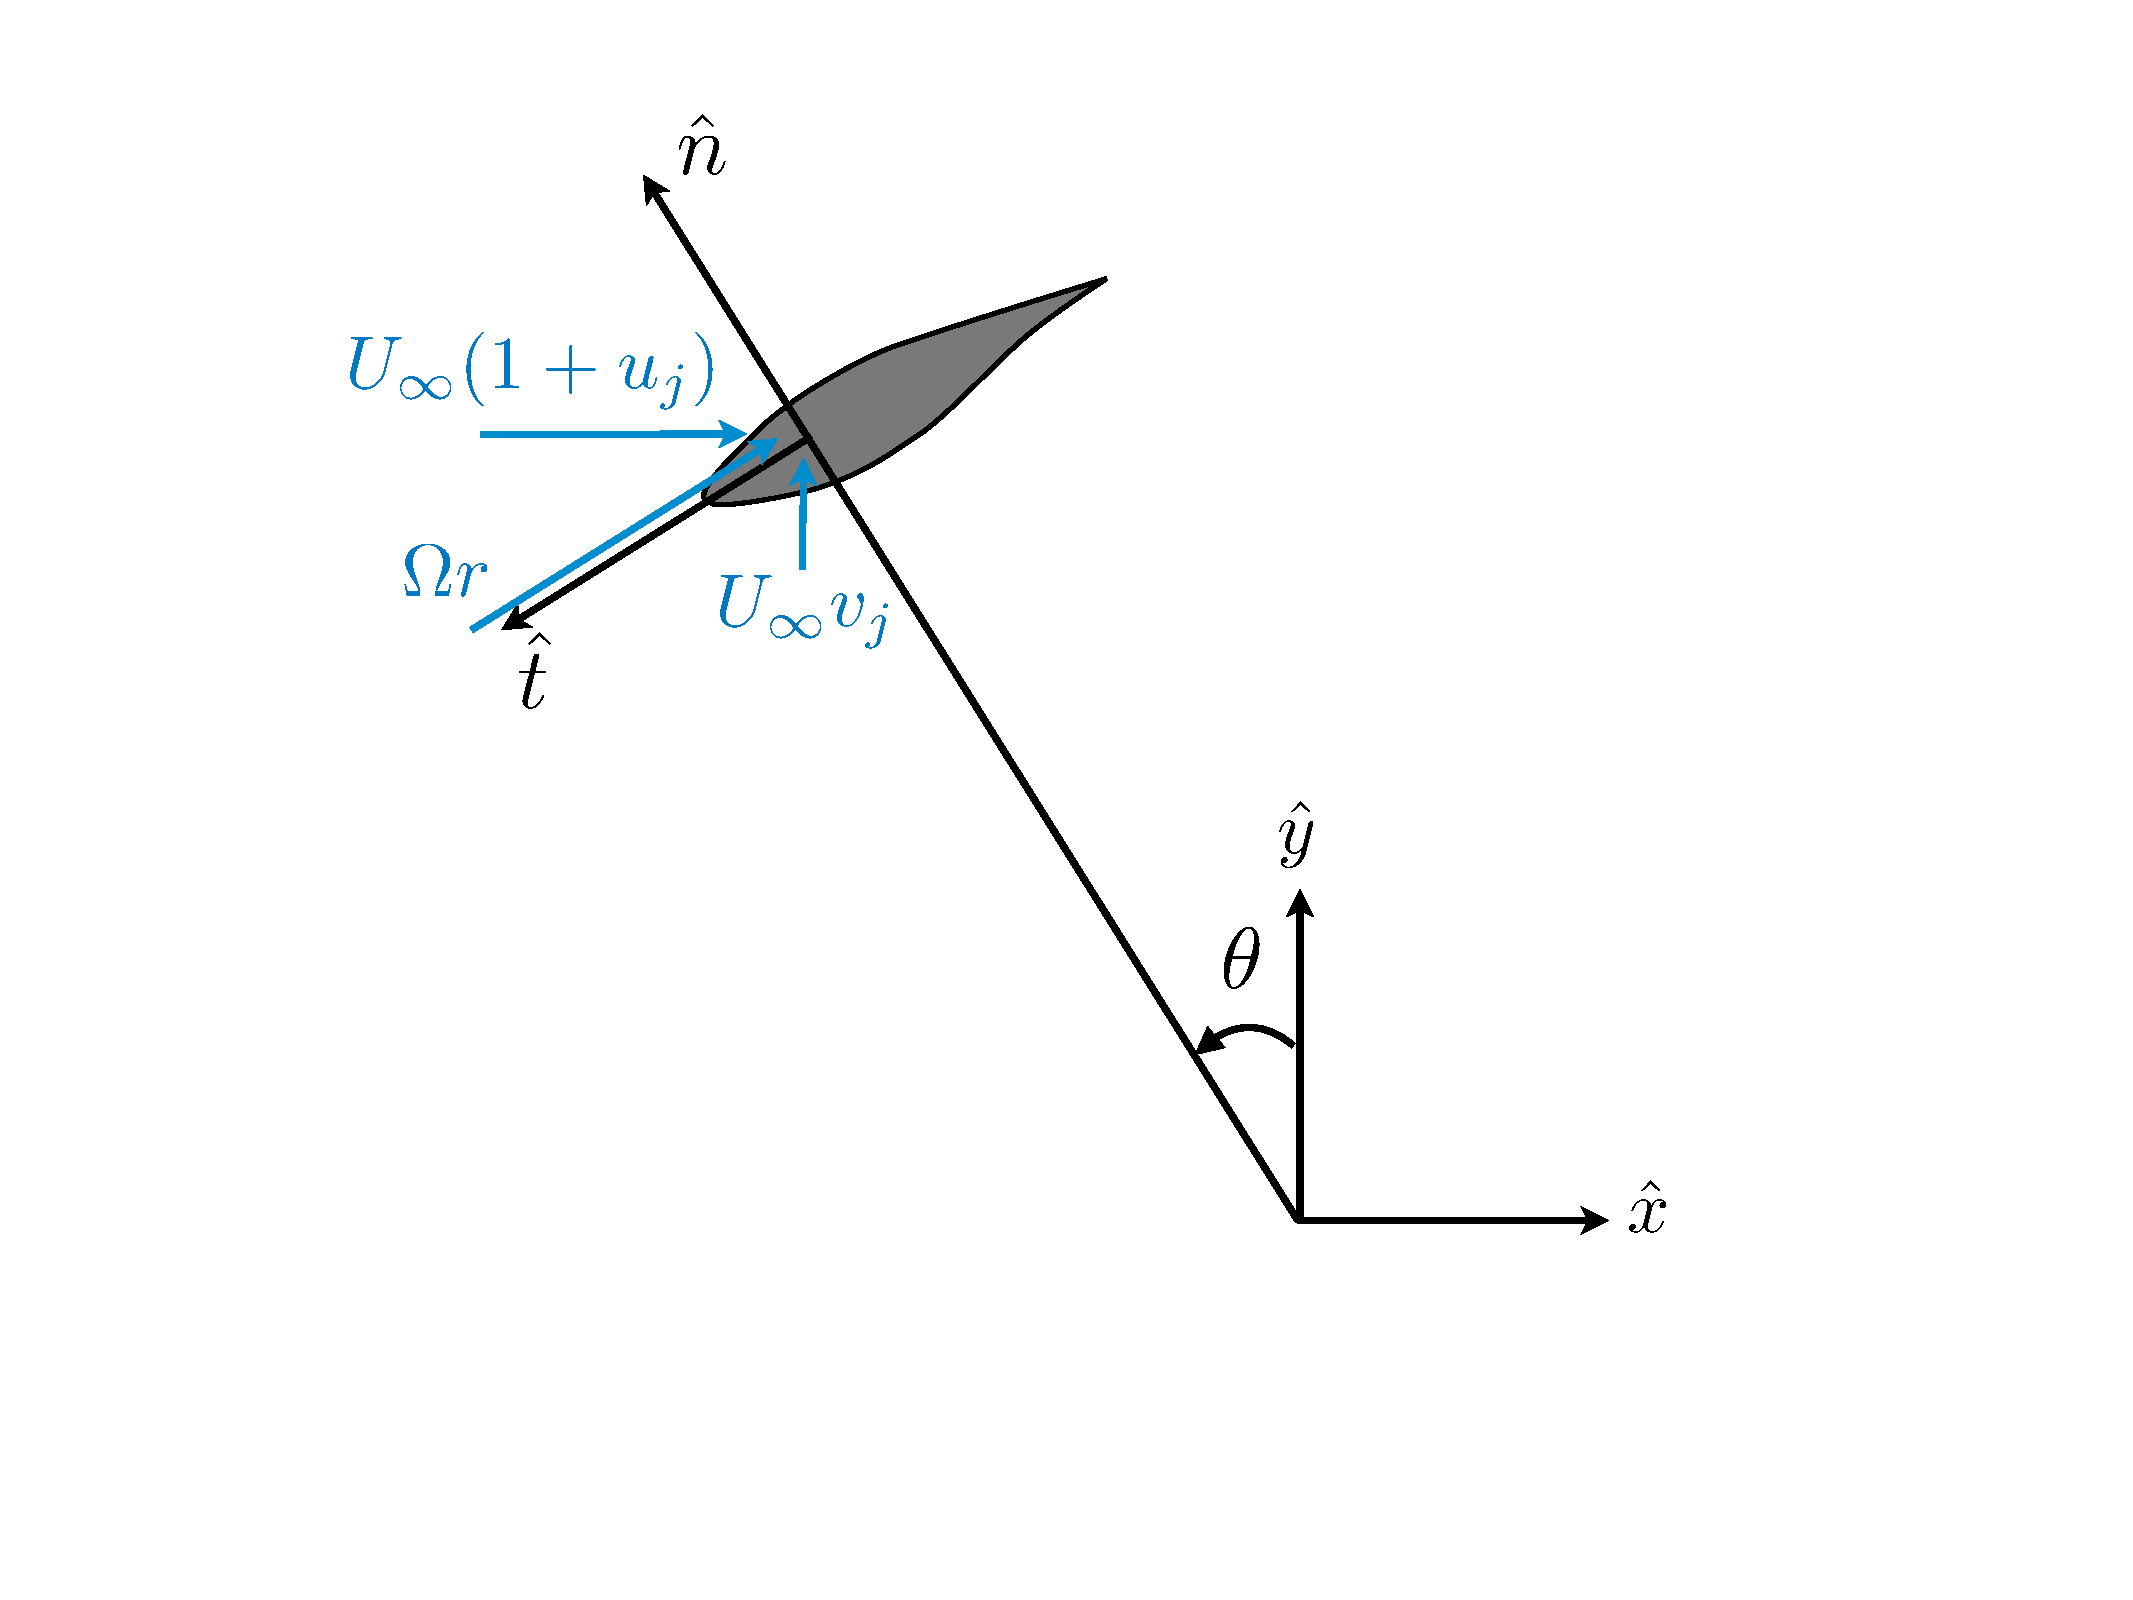
\includegraphics[width=3.5in]{images/velocity}
\caption{Relative components of velocity in the frame of the airfoil.}
\label{fig:velocity}
\end{center}
\end{figure}

Using the following coordinate transformations
\begin{align*}
 \hat{x} &= -\cos\theta\hat{t} - \sin\theta\hat{n}\\
 \hat{y} &= -\sin\theta\hat{t} + \cos\theta\hat{n}
\end{align*}
the velocity can be expressed in the $\hat{n}-\hat{t}$ plane as
\[ \vec{V}_j = \left[ - U_\infty(1+u_j) \sin\theta + U_\infty v_j \cos\theta\right]\hat{n} + \left[ - U_\infty(1+u_j) \cos\theta - U_\infty v_j \sin\theta -\Omega r \right]\hat{t} \]
These velocity components are depicted in Figure \ref{fig:components}.

\begin{figure}[htbp]
\begin{center}
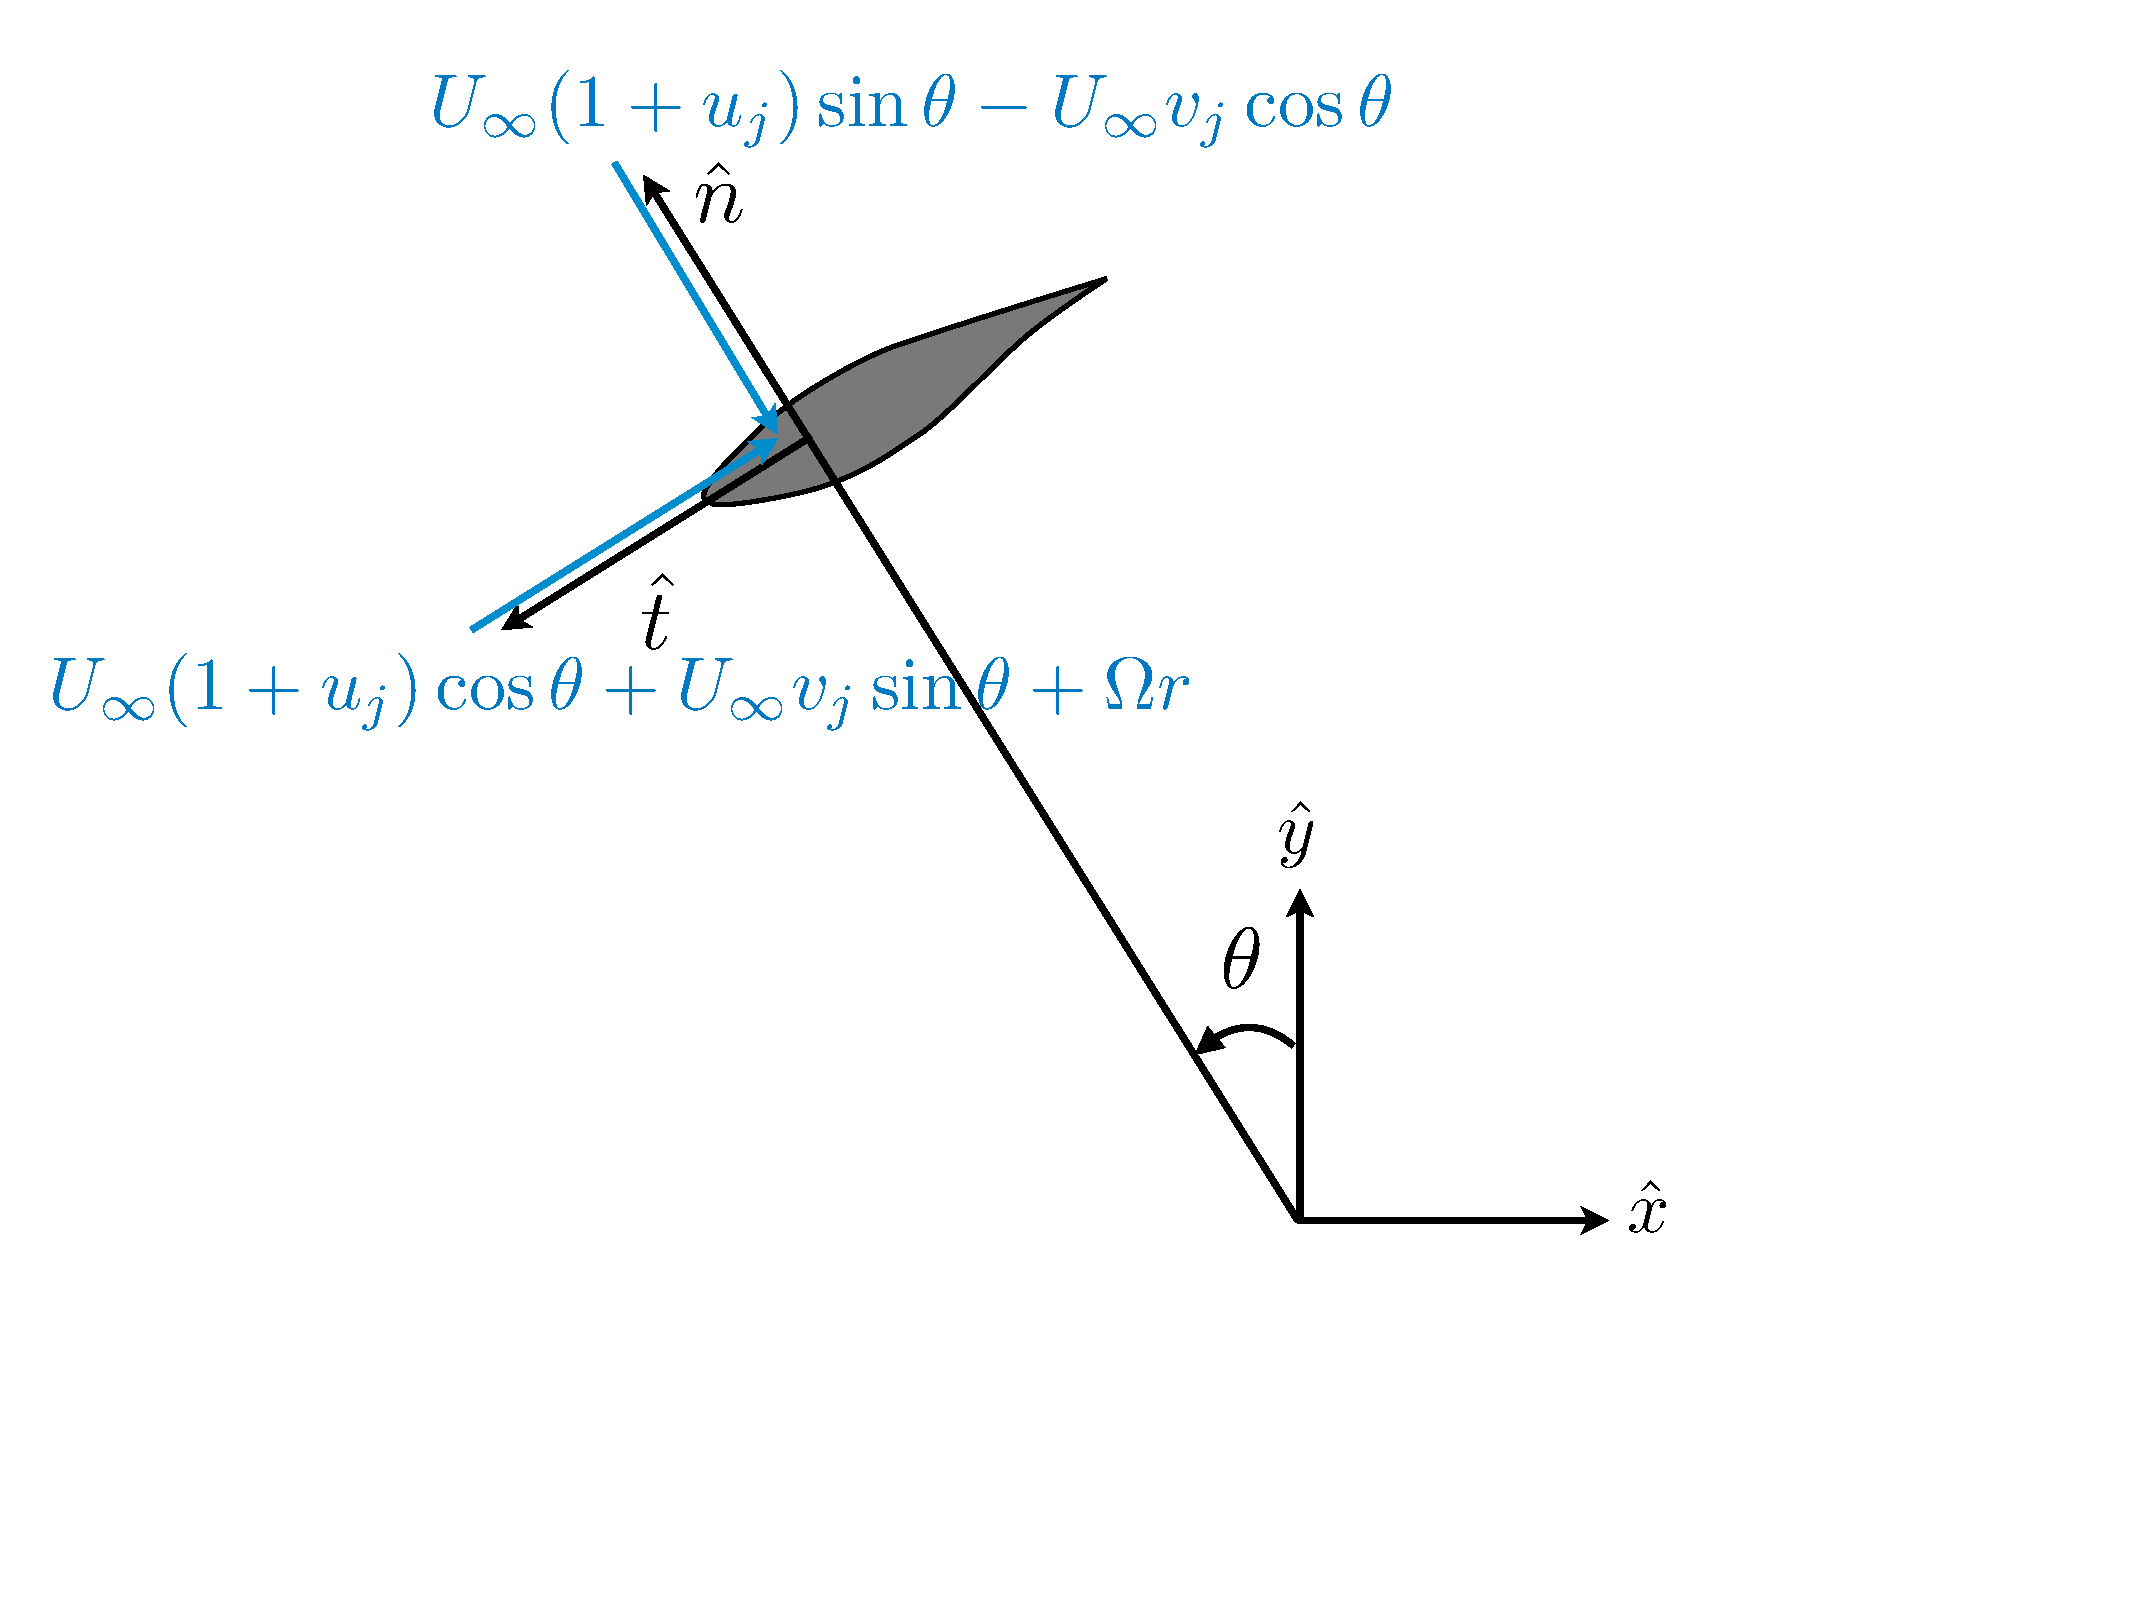
\includegraphics[width=3.5in]{images/components}
\caption{Componets of velocity resolved into $\hat{n}-\hat{t}$ plane.}
\label{fig:components}
\end{center}
\end{figure}

If we define the magnitudes
\begin{align*}
{V_n}_j &\equiv U_\infty(1+u_j) \sin\theta - U_\infty v_j \cos\theta\\
{V_t}_j &\equiv U_\infty(1+u_j) \cos\theta + U_\infty v_j \sin\theta +\Omega r
\end{align*}
then
\[ \vec{V}_j =  -{V_n}_j\hat{n} -{V_t}_j\hat{t} \]
and the magnitude of the local relative velocity and local inflow angle are
\begin{align*}
W_j &= \sqrt{{V_n}_j^2 + {V_t}_j^2}\\
\phi_j &= \tan^{-1}\left(\frac{{V_n}_j}{{V_t}_j}\right)
\end{align*}
the angle of attack, Reynolds number, and lift and drag coefficients can then be estimated as
\begin{equation}
  \begin{aligned}
\alpha_j &= \phi_j - \beta\\
Re_j &= \frac{\rho W_j c}{\mu}\\
{c_l}_j &= f(\alpha_j, Re_j)\\
{c_d}_j &= f(\alpha_j, Re_j)\\
\end{aligned}
\end{equation}
The normal and tangential forces are then
\begin{equation}
\begin{aligned}
{c_n}_j &= {c_l }_j\cos\phi_j + {c_d}_j\sin\phi_j \\
{c_t}_j &= {c_l }_j\sin\phi_j - {c_d}_j\cos\phi_j
\end{aligned}
\end{equation}
Because the blades are rotating we need to compute an azimuthally averaged value of the radial loading (recalling the sign convention for a positive radial loading is inward for loads the fluid produces on the VAWT)
\begin{equation}
  {F_r^\prime}_j = {c_n}_j \frac{1}{2}\rho W_j^2 c \frac{B \Delta\theta}{2\pi}
\end{equation}
Substituting into \eqref{eq:Qr} to find that the volume force can be expressed as
\begin{equation}
{Q_r}_j = {c_n}_j \frac{1}{2}\rho W_j^2 c \frac{B \Delta\theta}{2\pi} \frac{1}{r \Delta\theta} \frac{1}{\rho U_\infty^2}
\end{equation}
After simplification the volume force is
\begin{equation}
{Q_r}_j = \frac{Bc}{4\pi r}{c_n}_j \left(\frac{W_j}{U_\infty}\right)^2
\end{equation}
This expression is unmodified even when the blades are curved, because although the in-plane normal force varies with the cosine of the local curvature angle $\delta$, the area over which the force acts also varies with the cosine of the angle.

\subsection{Correction Factor}
Madsen notes that this linear solution produces good trends for the induced velocities, but is off in magnitude \cite{Madsen2013}.  For a uniform loading this linear solution can be shown to produce the following relationship between the thrust coefficient and the induction factor ($a = -u/U_\infty$).
\begin{equation}
  C_T = 4\ a_{linear}
\end{equation}

We can also use BEM theory to predict the thrust coefficient from the induction factor.  The solution depends on the region
\begin{equation}
C_T =
\begin{cases}
4 a (1-a)  & a \leq 0.4 \textrm{ (momentum)}\\
\frac{2}{9} (7a^2 - 2a + 4)  & 0.4 < a < 1 \textrm{ (empirical)}\\
4 a (a-1)  & a > 1 \textrm{ (propeller brake)}
\end{cases}
\label{eq:CT}
\end{equation}
In order to get the equivalent thrust coefficient we need to multiply our predicted induced velocities (and thus the thrust coefficient) by the correction factor $k_a = {C_T}_{linear} / C_T$
The correction factors become
\begin{equation}
k_a =
\begin{cases}
1/(1-a)  &  \textrm{ (momentum)}\\
(18 a)/(7a^2 - 2a + 4)  & \textrm{ (empirical)}\\
1/(a-1)  & \textrm{ (propeller brake)}
\label{eq:ka}
\end{cases}
\end{equation}
In order to determine the value of $a$ to use in the above equation we first find the thrust coefficient.  The instantaneous thrust coefficient can be found from \eqref{eq:xprime} normalizing by the dynamic pressure and the relevant area $2r$ (other dimension comes from the distributed loads being the force per unit length in the z-direction).
\begin{equation}
{C_T}_{inst} =  \left(\frac{W}{U_\infty}\right)^2  (c_n \sin\theta - c_t \frac{\cos \theta}{\cos\delta}) \frac{c}{2r}
\end{equation}
To get the total thrust coefficient we need to compute the azimuthal average
\begin{equation}
\begin{aligned}
  C_T &= \frac{B}{2\pi}\int_0^{2\pi} {C_T}_{inst}(\theta) d\theta \\
  &= \frac{Bc}{4\pi r}\int_0^{2\pi} \left(\frac{W}{U_\infty}\right)^2  (c_n \sin\theta - c_t \frac{\cos \theta}{\cos\delta}) d\theta
\end{aligned}
\end{equation}
From the thrust coefficient we can compute the expected induction factor by reversing \eqref{eq:CT}
\begin{equation}
a =
\begin{cases}
\frac{1}{2}\left(1 - \sqrt{1 - C_T}\right)  & C_T \leq 0.96 \textrm{ (momentum)}\\
\frac{1}{7}\left(1 + 3\sqrt{\frac{7}{2}C_T - 3}\right)  & 0.96 < C_T < 2 \textrm{ (empirical)}\\
\frac{1}{2}\left(1 + \sqrt{1 + C_T}\right)  & C_T > 2 \textrm{ (propeller brake)}
\end{cases}
\end{equation}
Finally, this induction factor allows us to compute the correction factor from \eqref{eq:ka}, which should multiply the induced velocities.

\subsection{Solution Procedure}

Note that the body forces are nonlinear functions of the induced velocities (i.e. $Q_r = f(w)$ where $w = [u; v]$).  However, the induced velocities are functions of the body forces (i.e, $w = k_a A Q_r$ where $A = [A_x; A_y]$).  This becomes a root finding problem for the induced velocities by solving  for the roots of the function
\begin{equation}
  f(w) = k_a A Q_r(w) - w
\end{equation}

If used as part of a dynamic simulation, we do not need to converge the velocities at each time step, but rather use the induced velocities from the previous time-step and simply update the new velocities as $w_{t+1} = k_a A Q_r(w_{t})$.  Recall that these velocities are normalized by the freestream velocity.

\section{Total Blade and Turbine Loads}
For either the double multiple streamtube method, or the actuator cylinder method, the two-dimensional surface swept out by the blades is discretized in both height and azimuthal location (\Cref{fig:grid}).  The three force components (radial, tangential, vertial) per unit length in the z-direction at each point can be expressed as (repeat of Eq. \eqref{eq:forces})
\begin{equation}
\begin{aligned}
  R^\prime &= -c_n \frac{1}{2} \rho W^2 c \\
  T^\prime &= c_t \frac{1}{2}\rho W^2 \frac{c}{\cos\delta } \\
  Z^\prime &= -c_n\frac{1}{2}\rho W^2 c \tan\delta
\end{aligned}
\end{equation}
 For each azimuthal station of interest, the solution is projected onto the instantaneous locations of the blade discretization.  For an unswept blade, this involves just a straightforward transfer of forces as the blade discretization would typically be exactly aligned with the surface discretization.  However, for swept blades, interpolation is necessary to resolve the forces along the curved blade path.  Furthermore, for a swept blade, the normal and tangential directions change along the blade path.  If each discretization point along the blade is at some azimuthal offset ($\Delta \theta$) from a reference point (e.g., relative to the the equatorial blade location), then the total normal force, tangential force, and torque produced by the blade are
\begin{equation}
\begin{aligned}
  R_{blade}(\theta) &= \int R^\prime(\theta + \Delta\theta) \cos(\Delta \theta) - T^\prime(\theta + \Delta\theta) \sin(\Delta \theta) dz \\
  T_{blade}(\theta) &= \int R^\prime(\theta + \Delta\theta) \sin(\Delta \theta) + T^\prime(\theta + \Delta\theta) \cos(\Delta \theta) dz \\
  Z_{blade}(\theta) &= \int Z^\prime(\theta + \Delta\theta) dz \\
  Q_{blade}(\theta) &= \int r T^\prime(\theta + \Delta\theta) dz
\end{aligned}
\end{equation}

\begin{figure}[htbp]
\begin{center}
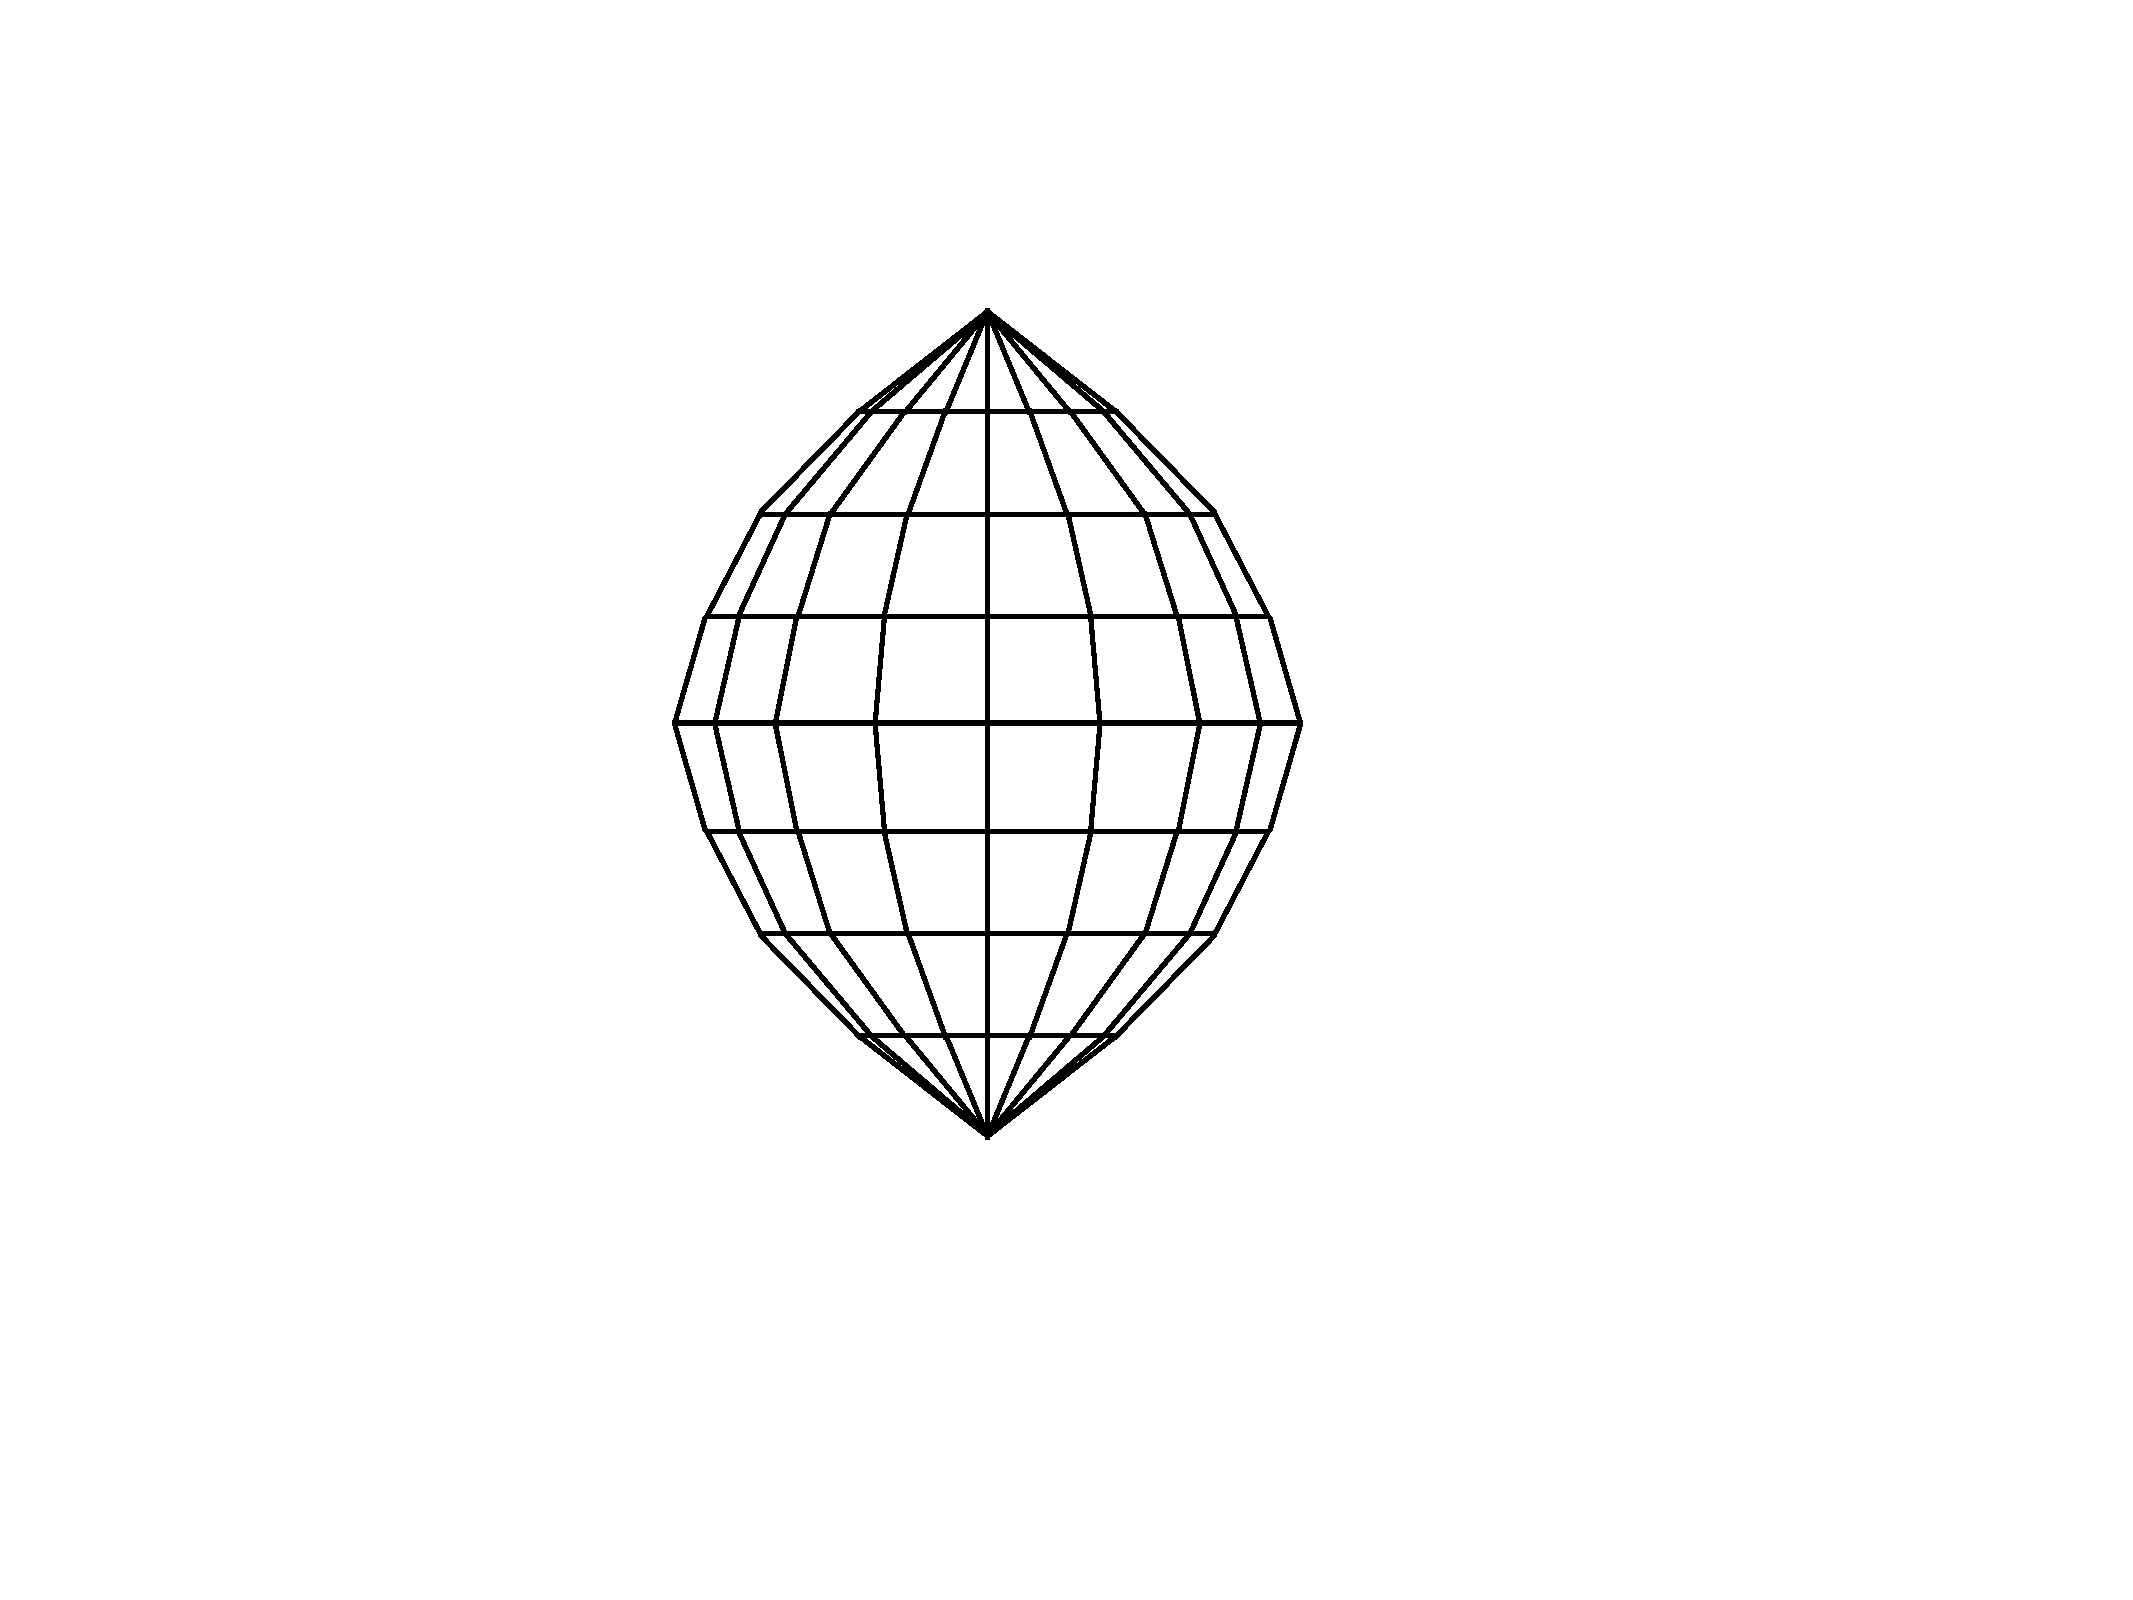
\includegraphics[width=1.5in]{images/grid}
\caption{Example two-dimensional discretization in height and azimuthal position of swept surface (side-view).}
\label{fig:grid}
\end{center}
\end{figure}

Now that the forces as a function of $\theta$ are known for one blade, the forces for all $B$ blades can be found.  We let $\Delta \Theta_j$ represent the offset of blade j relative to the first blade
\begin{equation}
\Delta\Theta_j = 2\pi (j-1) / B
\end{equation}
The resulting forces in the inertial frame (\Cref{fig:top}) are then
\begin{equation}
\begin{aligned}
  X_{all-blades}(\theta) &= \sum_{j=1}^B -R_{blade}(\theta + \Delta\Theta_j) \sin(\theta + \Delta\Theta_j) - T_{blade}(\theta + \Delta\Theta_j) \cos(\theta + \Delta\Theta_j) \\
  Y_{all-blades}(\theta) &= \sum_{j=1}^B R_{blade}(\theta + \Delta\Theta_j) \cos(\theta + \Delta\Theta_j) - T_{blade}(\theta + \Delta\Theta_j) \sin(\theta + \Delta\Theta_j) \\
  Z_{all-blades}(\theta) &= \sum_{j=1}^B Z_{blade}(\theta + \Delta\Theta_j)
\end{aligned}
\end{equation}
Finally, the power is given by averaging the torque across $\theta$
\begin{equation}
P = \Omega \frac{B}{2\pi} \int Q_{blade}(\theta) d\theta
\end{equation}


\bibliographystyle{aiaa}
\bibliography{~/Dropbox/NREL/Papers/wind}

\end{document}